\documentclass[oneside,letterpaper,titlepage]{article}
%\usepackage[ae,hyper]{/usr/lib/R/share/texmf/Rd}
\usepackage{makeidx}
\usepackage{graphicx}
\usepackage{natbib}
\usepackage[reqno]{amsmath}
\usepackage{amssymb}
\usepackage{verbatim}
\usepackage{epsf}
\usepackage{url}
\usepackage{html}
\usepackage{dcolumn}
\usepackage{longtable}
\usepackage{vmargin}
\usepackage{times}
\setpapersize{USletter}
\newcolumntype{.}{D{.}{.}{-1}}
\newcolumntype{d}[1]{D{.}{.}{#1}}
%\pagestyle{myheadings}
\htmladdtonavigation{
  \htmladdnormallink{%
    \htmladdimg{http://gking.harvard.edu/pics/home.gif}}
  {http://gking.harvard.edu/}}
\newcommand{\hlink}{\htmladdnormallink}

\bodytext{ BACKGROUND="http://gking.harvard.edu/pics/temple.setcounter"}
\setcounter{tocdepth}{3}

\newcommand{\MatchIt}{\textsc{MatchIt}}

\title{\MatchIt : Matching Software for Causal Inference} 

\author{Daniel E. Ho\thanks{J.D.\ candidate, Yale Law School, Ph.D.\ 
    candidate, Department of Government, Harvard University. (Center
    for Basic Research in the Social Sciences, 34 Kirkland, Cambridge
    MA 02138, USA;
    \href{http://www.people.fas.harvard.edu/\~deho}{http://www.people.fas.harvard.edu/\~\,deho},
    \href{mailto:Deho@Fas.Harvard.Edu}{Deho@Fas.Harvard.Edu}).}
\and %
Kosuke Imai\thanks{Assistant Professor, Department of Politics, Princeton
    University (Corwin Hall 041, Department of Politics, Princeton
    University, Princeton NJ 08544, USA;
    \href{http://www.princeton.edu/\~kimai}{http://www.princeton.edu/\~\,kimai},
    \href{mailto:KImai@Princeton.Edu}{KImai@Princeton.Edu}).}
\and %
Gary King\thanks{David Florence Professor of Government, Harvard
  University (Center for Basic Research in the Social Sciences, 34
  Kirkland Street, Harvard University, Cambridge MA 02138;
  \href{http://GKing.Harvard.Edu}{http://GKing.Harvard.Edu}, \href{mailto:King@Harvard.Edu}{King@Harvard.Edu}, (617)
  495-2027).}
\and %
Elizabeth A. Stuart\thanks{Ph.D.\ Candidate, Department of Statistics, Harvard
  University. (Science Center 702, One Oxford Street, Cambridge, MA
  02138, USA;
  \href{http://www.people.fas.harvard.edu/\~estuart}{http://www.people.fas.harvard.edu/\~\,estuart},
  \href{mailto:Stuart@Stat.Harvard.Edu}{Stuart@Stat.Harvard.Edu}).}}

\makeindex

\begin{document}
\maketitle

\begin{rawhtml}
<p>
  [Also available is a downloadable <a href="/matchit/docs/matchit.pdf">PDF</a>
  version of this entire document]
\end{rawhtml}

\tableofcontents

\section{Introduction}
\MatchIt\ implements the suggestions of Ho, Imai, King, and Stuart
(2004) for improving parametric statistical models by preprocessing
data with semi-parametric matching methods.  \MatchIt\ implements a wide
range of sophisticated matching methods, making it possible to greatly
reduce the dependence of causal inferences on commonly made, but
hard-to-justify, statistical modeling assumptions.  The software also
easily fits into existing research practices since, after
preprocessing with \MatchIt, researchers can use whatever parametric
model they would have used without \MatchIt, but produce inferences
with substantially more robustness and less sensitivity to modeling
assumptions.  Matched data sets created by \MatchIt\ can be entered
easily in \href{http://gking.harvard.edu/zelig/}{Zelig} for subsequent
parametric analyses.

% (\citealt{rubin74,RosRub83,RosRub84,Holland86}).  

\subsection{Software Requirements} 
\MatchIt\ works in conjunction with the R language and statistical
software, and will run on any platform where R is installed (Windows,
Unix, or Mac OS X).  R is available free for download at the
Comprehensive R Archive Network (CRAN) at
\href{http://www.r-project.org/}{http://www.r-project.org/}.
\MatchIt\ has been tested on R Version 1.9.0.

\subsection{Installing \MatchIt} 

There are two ways to install \MatchIt\: 

\begin{enumerate} 
\item For the easiest way to install \MatchIt\ for all platforms,
  type at the R prompt:
% We should change these addresses to Gary's site at some point
\begin{verbatim}
 > install.packages("matchit", 
           CRAN="http://www.people.fas.harvard.edu/~deho")
\end{verbatim}

  \noindent \MatchIt\ will proceed to automatically install itself onto
  your system.  During the process you may either decide to keep or
  discard the installation files, which will not affect the way
  \MatchIt\ runs.

\item Alternatively, you can install \MatchIt\ from a \textbf{local file}:
  \begin{enumerate} 
  \item \textbf{Unix} Shell:
    \begin{enumerate}
    \item Download the \texttt{matchit\_0.1-1.tar.gz} file from
      \url{http://www.people.fas.harvard.edu/~deho/src/contrib}
    \item In the Unix shell, install the package locally by typing:
\begin{verbatim}
% R INSTALL matchit_0.1-1.tar.gz   
\end{verbatim}
      from the directory where the file is located.
    \end{enumerate}
  \item \textbf{Windows or Mac} systems:
    \begin{enumerate}
    \item Download the \texttt{matchit\_0.1-1.zip} file from 
      \url{http://www.people.fas.harvard.edu/~deho/bin/windows/contrib/1.7/}
    \item In the R GUI click on the option under \texttt{Packages}
      to ``Install package(s) from local zip files...''
      Navigate to the location of \texttt{matchit\_0.1-1.zip} and click ``Open.''
    \end{enumerate}
  \end{enumerate}
\end{enumerate}

\subsection{Loading \MatchIt}
As with any R package, you have to load \MatchIt\ in order to use it.
You can do this for each R session by typing:
\begin{verbatim}
> library(matchit) 
\end{verbatim}
at the command prompt.  Alternatively, you can specify R to load
\MatchIt\ automatically at launch.  (This allows you to skip the step
of typing {\tt library(matchit)} at the beginning of every R session.)
 
To do this, edit the {\tt Rprofile} file located in the R program
subdirectory, e.g. \texttt{C:/R/rw1090/etc/}, for Windows systems and
the {\tt .Rprofile} file located in the home directory for Unix/Linux
and Mac OS X systems.  Using a text editor such as Windows notepad,
add the following line to the file:
\begin{verbatim}
options(defaultPackages = c(getOption("defaultPackages"), "matchit"))
\end{verbatim}
For this change to take effect, you need to restart R.

\subsection{Updating \MatchIt}
You may update to the most recent version of \MatchIt\ by typing the
following commands from your R session.

\begin{small}
\begin{verbatim}
> update.packages("matchit",CRAN="http://www.people.fas.harvard.edu/~deho")
> library(matchit) 
\end{verbatim}
\end{small} 

\section{A User's Guide by Examples}
\MatchIt\ attempts to balance the covariates of the treatment and
control units by allowing the user to specify the precise matching
algorithm.  The outcome analysis can then be performed on the matched
dataset, either via Zelig or any other routine in R.

We illustrate the basic capacities of \MatchIt\ through a series of
examples, all of which are contained in a demo script, which may be
run by: 

\begin{verbatim}
> demo(lalonde)
\end{verbatim}

\subsection{Notation}
Unless otherwise noted, let $i$ index the $n$ units in the dataset,
$n_1$ the number of treated units, $n_0$ the number of control units
(such that $n=n_0+n_1$), and $x_i$ some observed covariate vector for
unit $i$.  $T_i=1$ indicates that unit $i$ was assigned treatment, and
$T_i=0$ that unit $i$ was assigned control.  $Y_i(1)$ represents the
potential outcome of unit $i$ under treatment and $Y_i(0)$ the
potential outcome of unit $i$ under control.  $Y_i(1)$ and $Y_i(0)$
are jointly unobservable, so we only observe
$Y_i^{obs}=T_i(Y_i(1))+(1-T_i)(Y_i(0))$.

\subsection{The Lalonde Data}
For all of our examples, we use data from the job training program
analyzed in \citet{lalonde86} and \citet{DehWah99}.  A subsample of
the data consisting of the National Supported Work
Demonstration (NSW) treated group and the comparison sample from the Population
Survey of Income Dynamics (PSID) is included in \MatchIt, and the full
dataset is available at
\url{http://www.columbia.edu/~rd247/nswdata.html}.\footnote{\texttt{data(lalonde)}
  was created using \texttt{NSWRE74\_TREATED.TXT} and
  \texttt{CPS3\_CONTROLS.TXT} from this website.}

The variables in this dataset are in Table~\ref{dwvars} below.  One
causal effect of interest is the impact that participation in the job
training program, \texttt{treat==1}, had on real earnings in 1978,
\texttt{re78}, for those that participated in the program, i.e., the
average treatment effect on the treated (ATT):

\begin{equation}\label{re78eqn}
E(\text{re78}(\text{treat}=1) | \text{treat}=1) - E(\text{re78}(\text{treat}=0) | \text{treat}=1),
\end{equation}

\noindent where \texttt{re78(treat=1)} represents the potential
outcome under the treatment of the job program, and
\texttt{re78(treat=0)} under control.  To be clear, note that the
first expression in Equation~\ref{re78eqn} is \emph{observed}, whereas
the second expression is the \emph{unobserved} counterfactual of real
earnings if participants had not participated.  The same expression of
the ATT, in the notation that has been generally adopted, is:

\begin{equation}
E(Y_i(1) | T_i=1 ) - E(Y_i(0) | T_i=1).
\end{equation}

\begin{table}[h]
\label{dwvars}
\centering
\begin{tabular}{lp{3in}}
  \hline 
  \multicolumn{1}{l}{Name} & \multicolumn{1}{c}{Description} \\
  \hline
  \multicolumn{2}{l}{\textbf{Outcome ($Y$)}} \\ 
  \texttt{re78} & Real earnings (1978) \\\\
  \multicolumn{2}{l}{\textbf{Treatment Indicator ($T$)}} \\
  \texttt{treat} & Treated in job training program from March 1975-June
  1977 (1 if treated, 0 if not treated)
  \\ \\
  \multicolumn{2}{l}{\textbf{Pre-treatment Covariates ($X$)}} \\
  \texttt{age} & Age\\
  \texttt{educ} & Years of education \\
  \texttt{black} & Race black (1 if black, 0 otherwise) \\
  \texttt{hispan} & Race hispanic  (1 if Hispanic, 0 otherwise) \\
  \texttt{married} & Marital status (1 if married, 0 otherwise) \\
  \texttt{nodegree} & High school degree (1 if no degree, 0 otherwise)\\
  \texttt{re74} & Real earnings (1974) \\
  \texttt{re75} & Real earnings (1975) \\ 
  \hline
\end{tabular}\label{lalonde}
\caption{Description of Lalonde data}
\end{table}

\subsection{Exact Matching \label{exactm}}
The simplest version of matching is exact.  For example, to find exact
matches on race:\footnote{The examples in this document are for
  illustrative purposes only, and are not intended to obtain actual
  estimates of the average treatment effect, which would clearly
  require taking into account all pre-treatment variables.}

\begin{verbatim}
> data(lalonde)          #loads the example dataset
> foo1 <- matchit(treat ~ black + hispan, exact=TRUE, data=lalonde)
\end{verbatim}

\noindent \texttt{foo1} now contains all the information on the matched units.  The matching forms subclasses based on the covariates
in the formula portion of the \MatchIt\ call; within each subclass, all units have the same covariate values.  
To obtain basic information about the matching procedure: 

\begin{verbatim}
> print(foo1)
 
Assignment model specification:
matchit(formula = treat ~ black + hispan, data = lalonde, exact = TRUE)
 
Sample sizes for full and exactly matched data:
 
        Treated Control Total
Full        185     429   614
Matched     185     429   614
\end{verbatim} 
 
This returns the original call to \MatchIt.  We also see that all 185
treatment units were exactly matched to all 429 control units on race
covariates.  

We can obtain more information on the matching using the {\tt summary} command:

\begin{verbatim}
> summary(foo1)
 
Assignment model specification:
matchit(formula = treat ~ black + hispan, data = lalonde, exact = TRUE)
 
Summary of covariates for all data:
 
       Means Treated Means Control     SD T-stat    Bias
black        0.84324        0.2028 0.4894 19.344  1.7568
hispan       0.05946        0.1422 0.3220 -3.409 -0.3489
  
Sample sizes for full and exactly matched data:
 
        Treated Control Total
Full        185     429   614
Matched     185     429   614
 
Sample sizes by covariates:
 
  black hispan Treated Control Total
1     1      0     156      87   243
2     0      1      11      61    72
3     0      0      18     281   299
 
Number of units discarded:   0
\end{verbatim}

The means of the race variables ({\tt black} and {\tt
  hispan}) are quite different between the full treated and control groups, but within
each subclass formed by these two binary covariates the values of the
race variables of the treated and control units
are the same.  These two binary covariates form three subclasses, and
we see, for example, that 243 units (156 treated and 87 control) are
black and non-hispanic.

We can use the {\tt psclass} component of {\tt foo1} to identify which
units are in each subclass and to verify their covariate values.
To see ID numbers of the first 20 units in subclass 1 (``NSW'' refers
to the National Supported Work Demonstration participants):
\begin{verbatim}
> row.names(foo1$data)[foo1$psclass==1][1:20]
 [1] "NSW1"  "NSW3"  "NSW4"  "NSW5"  "NSW6"  "NSW7"  "NSW8"  "NSW9"  "NSW11"
[10] "NSW12" "NSW13" "NSW14" "NSW15" "NSW16" "NSW17" "NSW18" "NSW19" "NSW20"
[19] "NSW21" "NSW24"
\end{verbatim}

We can also confirm the covariate values of the units in each subclass.  For example, to see the covariate
values of the first 20 units in subclass 2 (``PSID''
refers to individuals in the Panel Survey of Income Dynamics):
\begin{verbatim}
> foo1$data[foo1$psclass==2,c("black", "hispan")][1:20,]
       black hispan
NSW2       0      1
NSW28      0      1
NSW44      0      1
NSW87      0      1
NSW100     0      1
NSW112     0      1
NSW129     0      1
NSW167     0      1
NSW173     0      1
NSW177     0      1
NSW180     0      1
PSID9      0      1
PSID16     0      1
PSID17     0      1
PSID21     0      1
PSID22     0      1
PSID28     0      1
PSID31     0      1
PSID40     0      1
PSID45     0      1
\end{verbatim}

\subsection{Exact Matching on All Covariates}

To match exactly on all covariates:

\begin{verbatim}
> foo <- matchit(treat ~ age + educ + black + hispan + married +
+                nodegree + re74 + re75, data=lalonde, exact=TRUE)

> summary(foo)
 
Assignment model specification:
matchit(formula = treat ~ age + educ + black + hispan + married +  
   nodegree + re74 + re75, data = lalonde, exact = TRUE)
 
Summary of covariates for all data:
 
         Means Treated Means Control        SD  T-stat     Bias
age          2.582e+01       28.0303    9.8812 -2.9911 -0.30945
educ         1.035e+01       10.2354    2.6283  0.5468  0.05496
black        8.432e-01        0.2028    0.4894 19.3443  1.75677
hispan       5.946e-02        0.1422    0.3220 -3.4091 -0.34890
married      1.892e-01        0.5128    0.4932 -8.5961 -0.82407
nodegree     7.081e-01        0.5967    0.4831  2.7127  0.24431
re74         2.096e+03     5619.2365 6477.9645 -7.2456 -0.72108
re75         1.532e+03     2466.4844 3295.6790 -3.2776 -0.29026
 
 
Sample sizes for full and exactly matched data:
 
        Treated Control Total
Full        185     429   614
Matched      13      12    25
 
Sample sizes by covariates:
 
  age educ black hispan married nodegree re74 re75 Treated Control Total
1  21   13     1      0       0        0    0    0       1       1     2
2  18   10     1      0       0        1    0    0       1       2     3
3  17   10     1      0       0        1    0    0       4       2     6
4  20   12     1      0       0        0    0    0       1       2     3
5  17    8     1      0       0        1    0    0       3       2     5
6  18   11     1      0       0        1    0    0       2       2     4
7  19   11     1      0       0        1    0    0       1       1     2
 
Number of units discarded:   0
\end{verbatim}


Hence out of the 185 observations in the NSW sample, only 25 units
have exact matches.

\subsection{Propensity Score Matching}
When exact matches do not exist, matching on the propensity score is a
common and useful alternative.  To propensity score match, with
pre-treatment covariates composed of real earnings in 1974 and 1975:

\begin{verbatim}
> foo2 <- matchit(treat ~ re74 + re75, data=lalonde)
\end{verbatim} 


\noindent You may again check basic statistics of the \MatchIt\ object by the
\texttt{print} command:

\begin{verbatim}
> print(foo2)
 
Assignment model specification:
matchit(formula = treat ~ re74 + re75, data = lalonde)
 
Summary of propensity score for full and matched samples:
 
        Means Treated Means Control      SD     T-stat       Bias
Full           0.3519        0.2795 0.11817  8.2436469  8.202e-01
Matched        0.3519        0.3520 0.08806 -0.0003493 -3.624e-05
 
Sample sizes:
 
        Treated Control Total
Full        185     429   614
Matched     185     185   370
 
\end{verbatim} 

We see that 185 control units were matched to the 185 treated units (a
``1-1'' match).  The average propensity scores in the matched treated
and control groups are much more similar than in the original groups,
with both groups having propensity score means of roughly $0.35$ in
the matched samples.  The {\tt summary} command gives further
information on the original and matched samples:

\begin{verbatim}
> summary(foo2)
 
Assignment model specification:
matchit(formula = treat ~ re74 + re75, data = lalonde)
 
Summary of covariates for all data:
 
       Means Treated Means Control        SD T-stat    Bias
pscore        0.3519        0.2795    0.1182  8.244  0.8202
re74       2095.5737     5619.2365 6477.9645 -7.246 -0.7211
re75       1532.0553     2466.4844 3295.6790 -3.278 -0.2903
 
Summary of covariates for matched data:
 
       Means Treated Means Control        SD     T-stat       Bias Reduction
pscore        0.3519        0.3520 8.806e-02 -0.0003493 -3.624e-05         1
re74       2095.5737     2040.3275 4.697e+03  0.1129664  1.131e-02         1
re75       1532.0553     1436.3806 2.849e+03  0.3225721  2.972e-02         1
 
Sample sizes:
 
        Treated Control Total
Full        185     429   614
Matched     185     185   370
 
Problematic covariates:
Number of units discarded:   0
\end{verbatim}

This reveals simple statistics of the propensity score and the
covariates used in the propensity score specification for the full and
matched samples, including t-statistics and balance bias statistics
used to assess whether there was a reduction in bias in the
covariates.\footnote{Balance bias statistics are a measure of how
  close covariates between treated and control groups are.  For a
  formal definition, see Subsection~\ref{cmd:sum}.}  All three
variables (propensity score, 1974 income, and 1975 income) had
reductions in bias due to the matching.  For example, the original
bias in 1974 income was $-0.72$ standard deviations, but is only
$0.011$ standard deviations in the matched samples.  More
specifically, job training participants on average earned roughly
\$3,523 less in 1974 and \$934 less in 1975 than non-participants,
significant differences with t-statistics of -7.25 and -3.28,
respectively.  In the matched sample, the earnings difference is only
\$56 (t-statistic=0.11) in 1974 and \$96 (t-statistic=0.32) in 1975.
This one-to-one matching algorithm has thus chosen 185 control
individuals who do look very similar to the treated group on the
covariates used in the matching process (1974 income and 1975 income).

The \texttt{summary} command will additionally report (a) the original
call of the \MatchIt\ object, (b) whether there are any ``Problematic
covariates'' that may still be imbalanced in the assignment
model,\footnote{A variable is considered ``problematic'' when the
  absolute value of the t-statistic in the matched sample exceeds 2,
  or when the absolute balance bias is greater in the matched sample
  than in the full sample.} and (c) how many units were discarded due
to the \texttt{discard} option (described below).  In this case there
were no units discarded and no ``problematic covariates.''

For further information on the balance in the full and matched samples
we can use the {\tt verbose=T} option with {\tt summary}, which
shows the balance of all squares and interactions of the covariates
used in the matching procedure.  This is helpful for diagnosing whether balance across matched
pairs has been attained.  Significant differences in higher order
interactions usually are a good indication that the assignment model
needs to be respecified, as discussed in Section \ref{pscorespec}.

\begin{verbatim}
> summary(foo2, verbose=T)
 
Assignment model specification:
matchit(formula = treat ~ re74 + re75, data = lalonde)
 
Summary of covariates and interactions for all data:
 
              Means Treated Means Control        SD  T-stat     Bias
pscore            3.519e-01     2.795e-01 1.182e-01  8.2436  0.82019
re74              2.096e+03     5.619e+03 6.478e+03 -7.2456 -0.72108
re75              1.532e+03     2.466e+03 3.296e+03 -3.2776 -0.29026
pscorexpscore     1.316e-01     9.312e-02 5.896e-02  8.5621  0.82170
pscorexre74       3.284e+02     7.620e+02 6.627e+02 -8.1426 -0.74246
pscorexre75       3.819e+02     4.960e+02 6.953e+02 -1.8020 -0.15444
re74xre74         2.814e+07     7.756e+07 1.353e+08 -4.5738 -0.43306
re74xre75         1.312e+07     2.543e+07 5.354e+07 -2.6991 -0.24252
re75xre75         1.265e+07     1.690e+07 4.478e+07 -0.9365 -0.07568
 
Summary of covariates and interactions for matched data:
 
              Means Treated Means Control        SD     T-stat       Bias
pscore            3.519e-01     3.520e-01 8.806e-02 -0.0003493 -3.624e-05
re74              2.096e+03     2.040e+03 4.697e+03  0.1129664  1.131e-02
re75              1.532e+03     1.436e+03 2.849e+03  0.3225721  2.972e-02
pscorexpscore     1.316e-01     1.316e-01 4.675e-02  0.0139071  1.444e-03
pscorexre74       3.284e+02     3.340e+02 5.772e+02 -0.0927353 -9.542e-03
pscorexre75       3.819e+02     3.959e+02 6.999e+02 -0.1916425 -1.891e-02
re74xre74         2.814e+07     2.442e+07 1.001e+08  0.3570086  3.261e-02
re74xre75         1.312e+07     8.919e+06 4.064e+07  0.9939819  8.270e-02
re75xre75         1.265e+07     7.942e+06 4.229e+07  1.0720362  8.410e-02
              Reduction
pscore                1
re74                  1
re75                  1
pscorexpscore         1
pscorexre74           1
pscorexre75           1
re74xre74             1
re74xre75             1
re75xre75             0
 
Sample sizes:
 
        Treated Control Total
Full        185     429   614
Matched     185     185   370
 
Problematic covariates:
Number of units discarded:   0
\end{verbatim}

We can also check the propensity score and covariate distribution with
diagnostic plots, which are depicted in Figure~\ref{f2diags}.  These
plot functions are interactive.  For example, the first menu asks
whether you would like to see density estimates of the propensity
scores.  Inputting \texttt{1} will yield the left-hand panel in
Figure~\ref{f2diags}.

\begin{verbatim}
> plot(foo2)
  Choices
0 No     
1 Yes    
Would you like to see density estimates of the propensity scores?
\end{verbatim}

The density curves overlay control and treatment units for full and
matched samples.  Next, the menu will prompt you whether you would
like to see jitter plots of the propensity scores.

\begin{verbatim}
Would you like to see density estimates of the propensity scores?1
  Choices
0 No     
1 Yes    
Would you like to see a jitterplot of the propensity scores?
\end{verbatim}

Entering a \texttt{1} also reveals instructions on how to
interactively identify particular units, which may be useful for
identifying particular outliers: 

\begin{verbatim}
[1] "To identify the units, use first mouse button; to stop, use
second."
\end{verbatim}

Clicking the first mouse button near the units will bring up the
observation name specified in the data frame.  You may end this by
clicking the second mouse button.

Lastly, the \texttt{plot} command allows you to plot density estimates
for any covariates and their interactions:\footnote{Note that when
  subclassification is specified, the \texttt{plot} command
  additionally permits plotting density estimates of any covariates
  within a particular subclass.}

\begin{verbatim}
  Choices         
0 No              
1 Yes :  pscore   
2 Yes :  re74     
3 Yes :  re75     
4 Yes :  re74xre74
5 Yes :  re74xre75
6 Yes :  re75xre75
Would you like to see density estimates of any other covariates?
\end{verbatim}

\begin{figure}[ph]
  \begin{center}
%    \rotatebox{270}{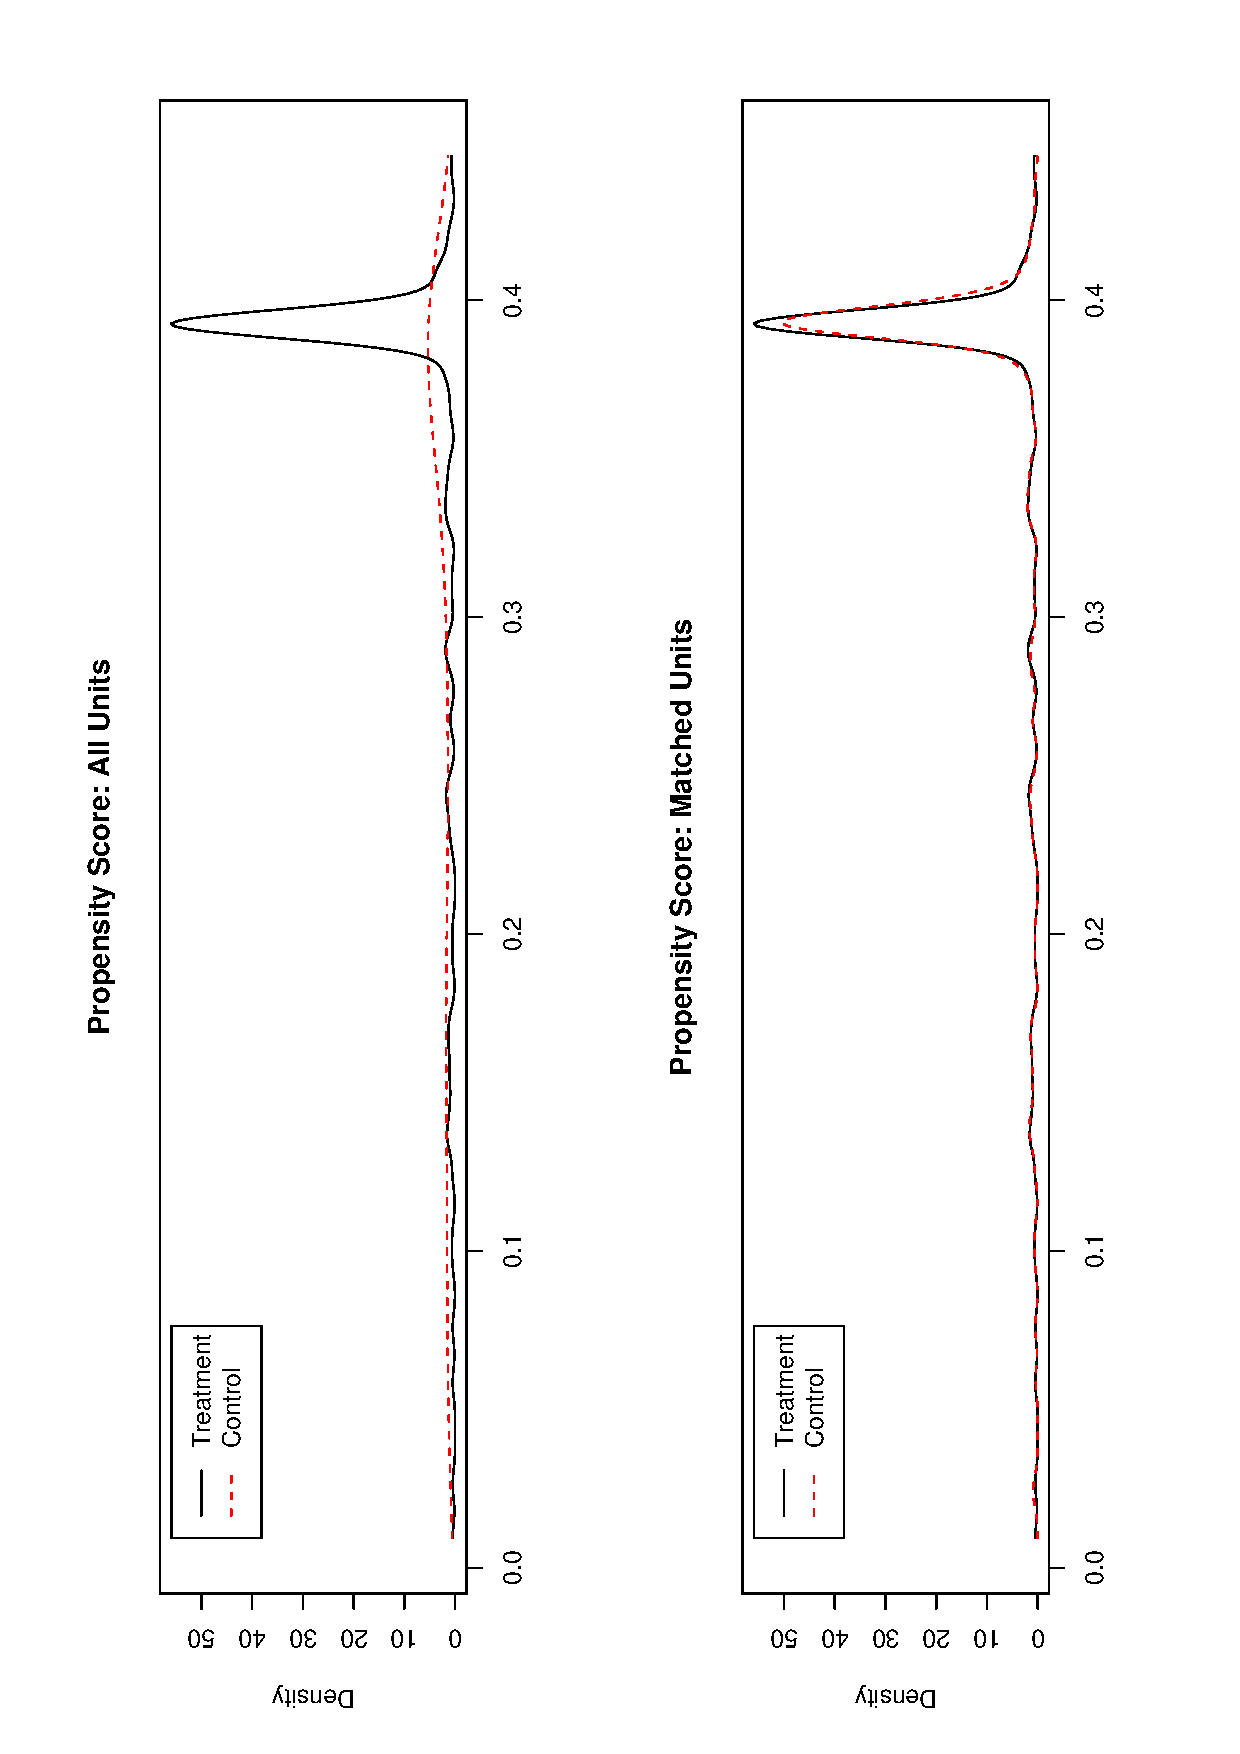
\includegraphics[height=2.35in,angle=0]{figs/f2figa}}
%    \rotatebox{270}{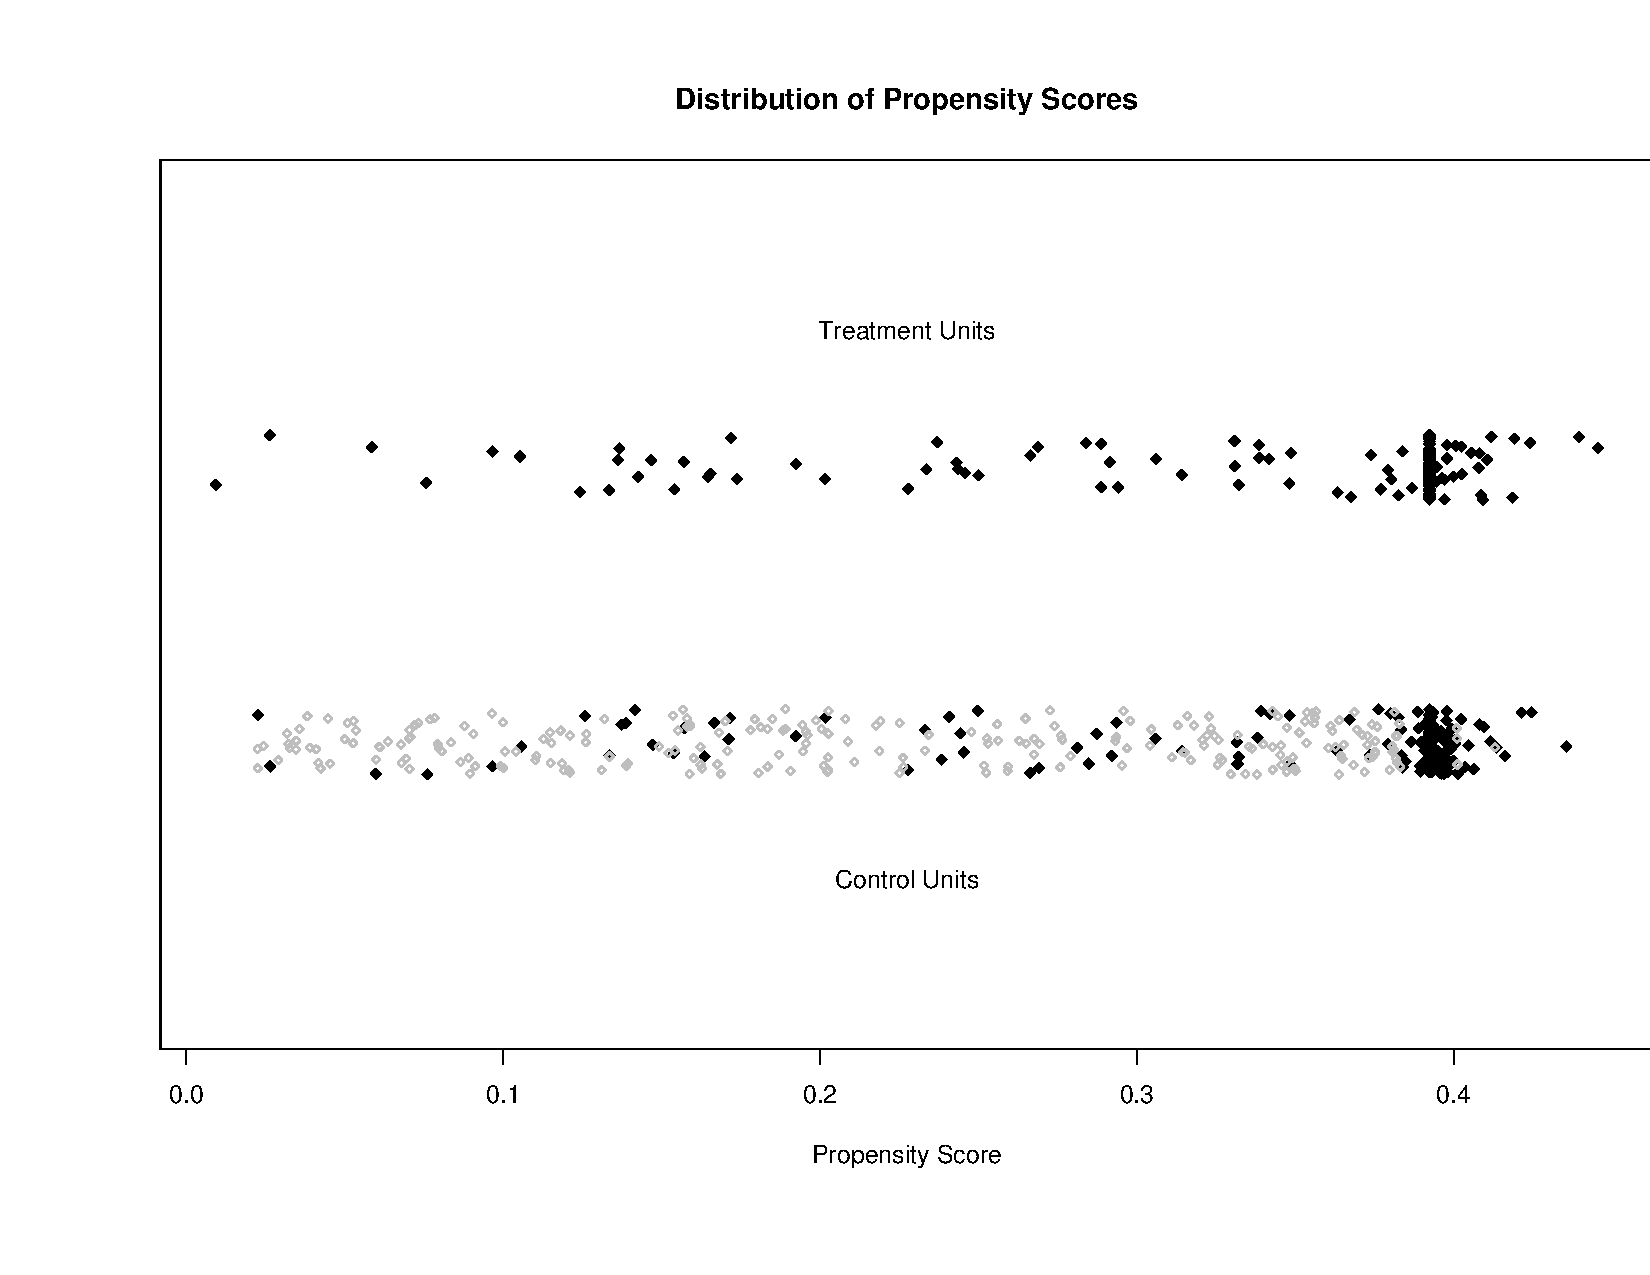
\includegraphics[height=2.35in,angle=0]{figs/f2figb}}
    \rotatebox{270}{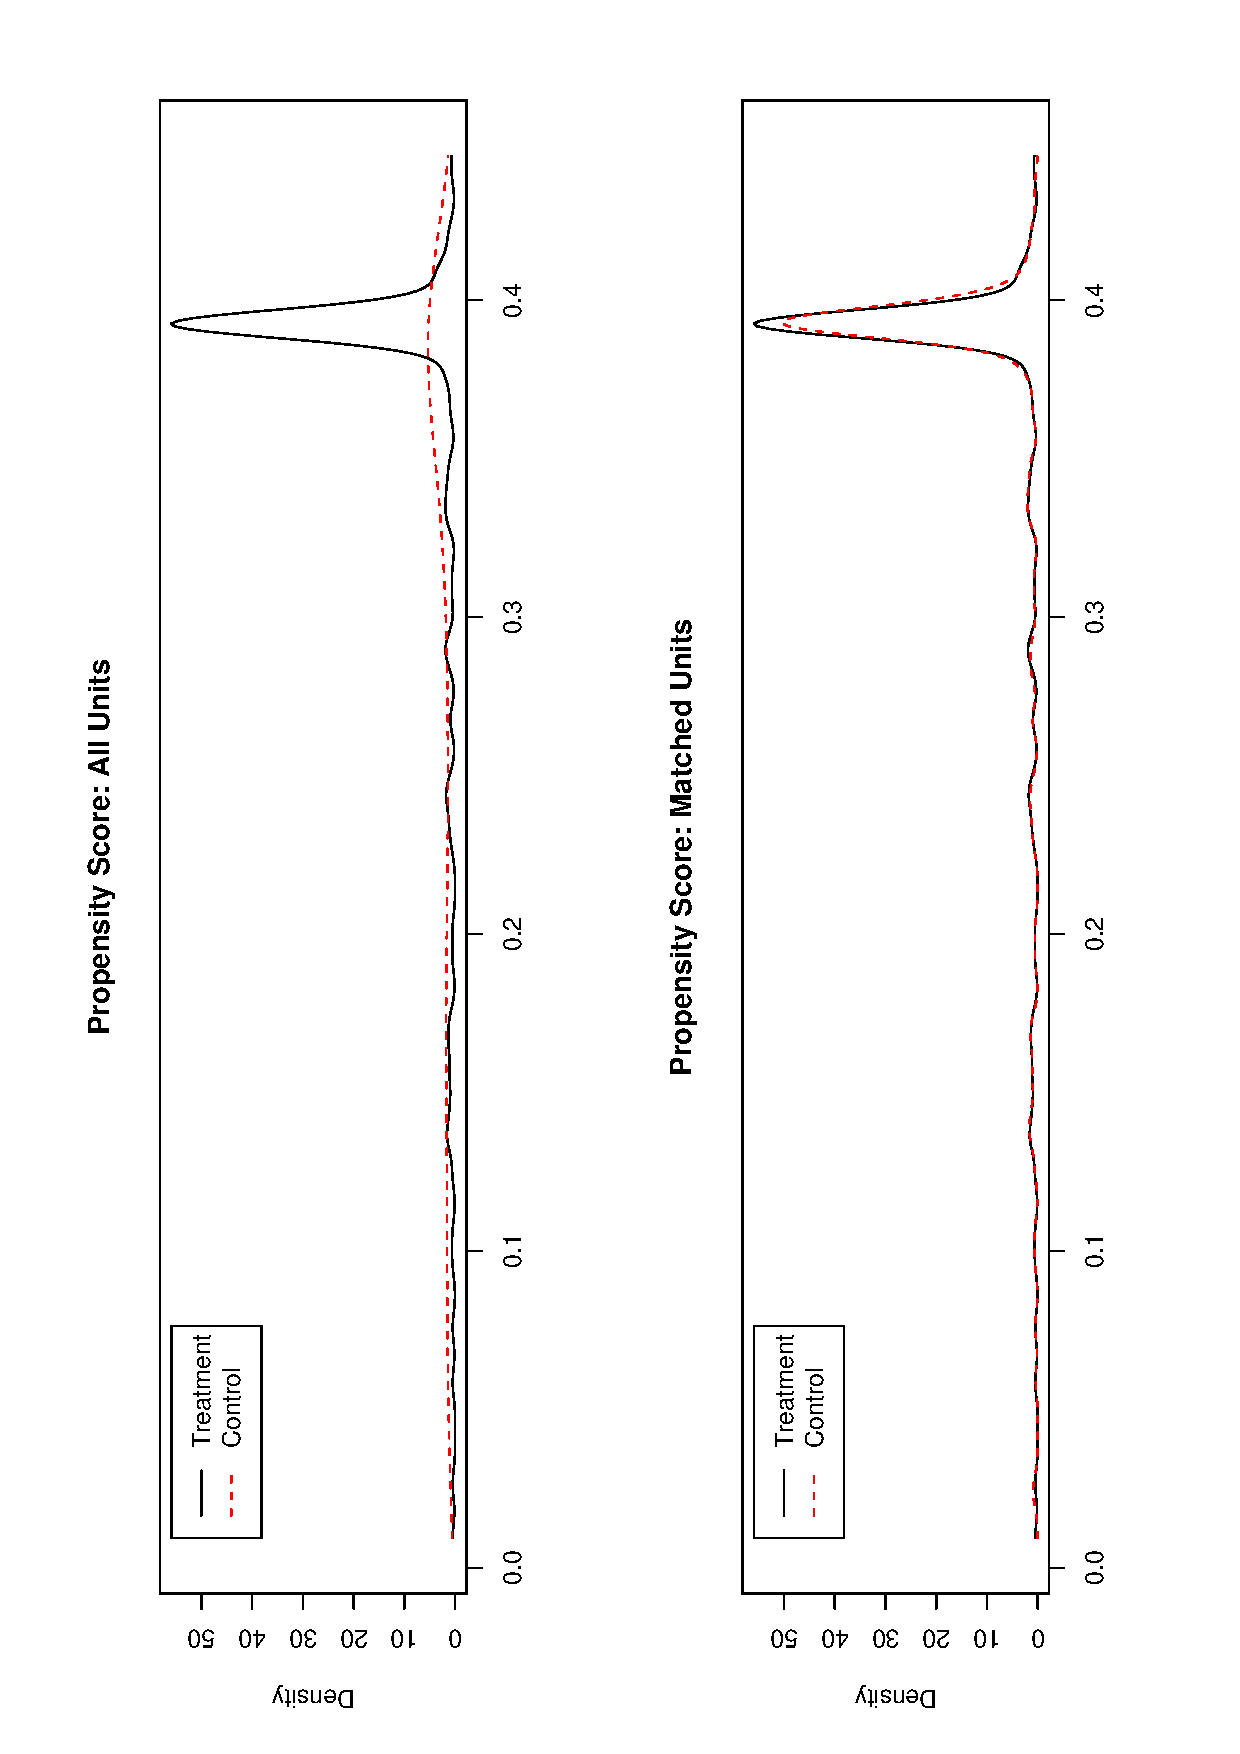
\includegraphics[height=4in,angle=0]{figs/f2figa}}
    \rotatebox{270}{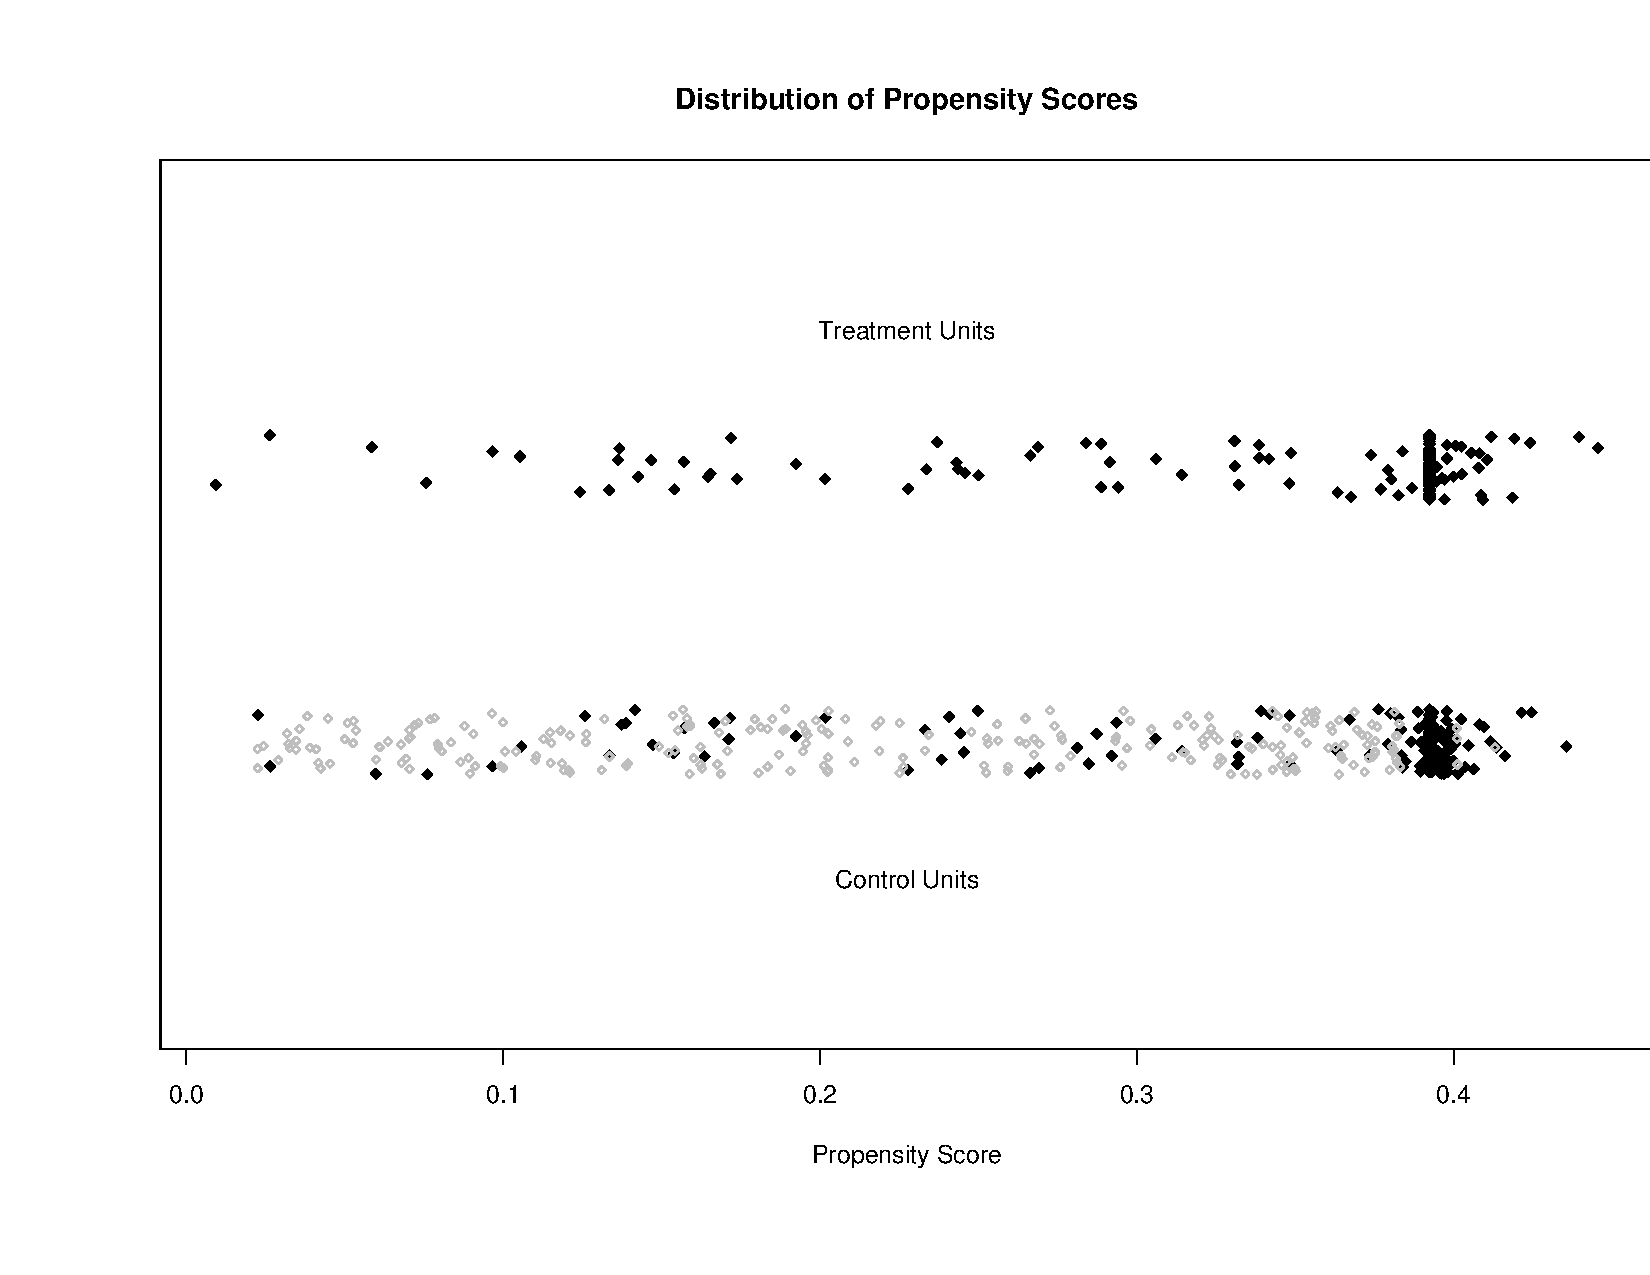
\includegraphics[height=4in,angle=0]{figs/f2figb}}
    \hfill
    \caption{Sample interactive diagnostic graphs}
    \label{f2diags}
  \end{center}
\end{figure}

Examining these graphs in Figure~\ref{f2diags}, we see that the
matched samples are very well matched on the propensity score, with
very similar distributions in the matched treated and control groups.

\subsection{Propensity Score Matching with Exact Restriction}

Now suppose we wanted to match on a propensity score specification
with real earnings in 1974 and 1975, as well as exact match on race:

\begin{verbatim}
> foo3 <- matchit(treat ~ re74 + re75, exact=c("black","hispan"),
  data=lalonde)
> print(foo3)
 
Assignment model specification:
matchit(formula = treat ~ re74 + re75, data = lalonde, 
   exact = c("black","hispan"))
 
 
Summary of propensity score for full and matched samples:
    
        Means Treated Means Control      SD T-stat   Bias
Full           0.3519        0.2795 0.11817  8.244 0.8202
Matched        0.3851        0.3349 0.08021  5.018 1.1226
 
Sample sizes:
 
        Treated Control Total
Full        185     429   614
Matched     116     116   232
\end{verbatim}

Exact matches on race were found for only 116 of the treated units,
and so there are 116 treated and 116 control units in the matched
samples.  We can quickly verify that the race variables in the matched
samples are the same:

\begin{verbatim}
> sum.foo3 <- summary(foo3)
> sum.foo3$sum.all[c("hispan","black"),]
       Means Treated Means Control        SD    T-stat       Bias
hispan    0.05945946     0.1421911 0.3219967 -3.409136 -0.3488957
black     0.84324324     0.2027972 0.4894132 19.344264  1.7567745
> sum.foo3$sum.matched[c("hispan","black"),]
       Means Treated Means Control        SD T-stat Bias Reduction
hispan    0.09482759    0.09482759 0.2936101      0    0         1
black     0.75000000    0.75000000 0.4339489      0    0         1
\end{verbatim}

The command {\tt summary(foo3)\$sum.all} gives a summary of the
covariates before matching, whereas {\tt summary(foo3)\$sum.matched}
gives the comparable summaries on the matched samples. Before
matching, 84\% of participants were black, compared to only 20\% of
the non-participants.  In the matched samples, black participants and
non-participants comprise 75\% of the observations.

It is easy to extract the matched subsetted data using the {\tt
  match.data} command.  The following three commands output the full
matched data set, the matched treated group, and the matched control
group, respectively:

\begin{verbatim}
dta.matched <- match.data(foo3)
dta.treated <- match.data(foo3, group = "treat")
dta.control <- match.data(foo3, group = "control")
\end{verbatim}

We can examine which units were matched to which using the {\tt
  match.matrix} output:
\begin{verbatim}
> foo3$match.matrix
            V1
NSW1   PSID406
NSW2   PSID385
NSW3   PSID388
NSW4   PSID326
NSW5   PSID337
NSW6   PSID376
NSW7   PSID134
NSW8   PSID355
NSW9      <NA>
NSW10  PSID422
...  
\end{verbatim}

The unit numbers on the left are the treated units; the units in the
2nd column are the controls matched to each treated unit.  For
example, PSID Unit 406 was matched to NSW Unit 1.  NSW Unit 9 did not
have a match.  We can verify that the matched pairs have identical race values 
(\texttt{black} and \texttt{hispan}):

\begin{verbatim}
> lalonde[c("NSW1", "PSID406"), c("black", "hispan")]
        black hispan
NSW1        1      0
PSID406     1      0

> lalonde[c("NSW2", "PSID385"), c("black", "hispan")]
        black hispan
NSW2        0      1
PSID385     0      1
\end{verbatim}


\subsection{Replication of Dehejia \& Wahba}

The following line replicates the matching algorithm of Table 2
(column 10, row 4) of \citet{DehWah99}:

\begin{verbatim}
> data(lalonde)                 #calls the Lalonde data
> foo <- matchit(treat ~ age + I(age^2) + educ + I(educ^2) + black +
  hispan + married + nodegree + re74  + I(re74^2) + re75 + I(re75^2) +
  I(as.numeric(re74==0)) + I(as.numeric(re75==0)), data=lalonde,
  replace=1,discard=1)
\end{verbatim}

Note that the only differences between this and the earlier propensity
score matching example are: (a) the number of covariates used, (b) the
\texttt{discard} option (which drops control units outside the support
of the treated group's propensity scores, and (c) matching with
replacement.

\subsection{Non-matched and Discarded Units}
The output objects \texttt{in.sample} and \texttt{psweights} give you
all the information about non-matched and discarded units.
\texttt{in.sample} is a logical vector of length $n$ that indicates whether each unit
was discarded due to the common support conditions (the
\texttt{discard} option), while \texttt{psweights} gives information
on whether each unit was matched.  If, for observation $i$,
\texttt{in.sample}[i] is TRUE and \texttt{psweights}[i] is $0$, then
unit $i$ was eligible for matching but not used.  If
\texttt{in.sample}[i] is FALSE, then \texttt{psweights}[i] will be $0$.

For example, suppose we use the assignment model from above:

\begin{verbatim}
> foo <- matchit(treat ~ age + I(age^2) + educ + I(educ^2) + black +
  hispan + married + nodegree + re74  + I(re74^2) + re75 + I(re75^2) +
  I(as.numeric(re74==0)) + I(as.numeric(re75==0)), data=lalonde,
  replace=1,discard=1)
\end{verbatim}

We can tell which units were discarded because of support conditions:

\begin{verbatim}
> foo$in.sample[!foo$in.sample]
   NSW5    NSW8   NSW51   NSW62   NSW63   NSW66   NSW71  NSW109  NSW136  NSW151
  FALSE   FALSE   FALSE   FALSE   FALSE   FALSE   FALSE   FALSE   FALSE   FALSE
 NSW164  NSW178   PSID3  PSID11  PSID16  PSID34  PSID39  PSID40  PSID44  PSID47
  FALSE   FALSE   FALSE   FALSE   FALSE   FALSE   FALSE   FALSE   FALSE   FALSE
...
\end{verbatim}

And we can also tell which units were not matched despite meeting
support conditions:

\begin{verbatim}
> foo$psweights[foo$in.sample & foo$psweights==0]
  PSID1   PSID2   PSID4   PSID5   PSID7   PSID9  PSID12  PSID13  PSID14  PSID18
      0       0       0       0       0       0       0       0       0       0
 PSID19  PSID20  PSID21  PSID22  PSID23  PSID24  PSID25  PSID26  PSID28  PSID29
      0       0       0       0       0       0       0       0       0       0
...
\end{verbatim}

One could further wonder how the discarded units differ from the
treated units in the NSW experiment:

\begin{verbatim}
> sdisc <- apply(lalonde[!foo$in.sample,],2,mean) #taking column-wise means
> streat <- apply(lalonde[lalonde$treat==1,],2,mean)
> round(rbind(sdisc,streat),2) #rounding
       treat   age  educ black hispan married nodegree    re74    re75    re78
sdisc    0.1 35.59  9.94  0.13   0.05    0.70     0.58 7484.53 2309.50 7760.00
streat   1.0 25.82 10.35  0.84   0.06    0.19     0.71 2095.57 1532.06 6349.14
\end{verbatim}

The units that were discarded because of support conditions were on
average about ten years older than the treated units, much less
likely to be black, more likely to be married, more likely to
have high school degrees, and had much higher income, particularly in
1974.

We can also use the {\tt psweights} output to examine how many times
each control unit was matched (when matching with replacement).
Printing out {\tt psweights} shows the weights themselves. Each
matched treated unit has a weight of one, whereas each matched control
unit has a weight proportional to the number of times it was matched:

\begin{verbatim}
> print(foo$psweights[foo$data$treat==1][1:10])
 NSW1  NSW2  NSW3  NSW4  NSW5  NSW6  NSW7  NSW8  NSW9 NSW10
    1     1     1     1     0     1     1     0     1     1

> print(foo$psweights[foo$data$treat==0][1:20])
    PSID1     PSID2     PSID3     PSID4     PSID5     PSID6     PSID7     PSID8
0.0000000 0.0000000 0.0000000 0.0000000 0.0000000 1.1271676 0.0000000 2.6300578
    PSID9    PSID10    PSID11    PSID12    PSID13    PSID14    PSID15    PSID16
0.0000000 0.3757225 0.0000000 0.0000000 0.0000000 0.0000000 0.3757225 0.0000000
   PSID17    PSID18    PSID19    PSID20
0.7514451 0.0000000 0.0000000 0.0000000
\end{verbatim}

NSW Unit 8 was not matched and thus has a weight of 0.  We need to
re-scale the control unit weights to see how many times each control
was matched.  The sum of the control group weights equals the
number of uniquely matched control units, so we re-scale by the number
of treated units matched divided by the number of control units
matched:

\begin{verbatim}
> print((foo$psweights[foo$data$treat==0]*sum(foo$psweights[foo$data$treat==1])/
  sum(foo$psweights[foo$data$treat==0]))[1:20])
 PSID1  PSID2  PSID3  PSID4  PSID5  PSID6  PSID7  PSID8  PSID9 PSID10 PSID11
     0      0      0      0      0      3      0      7      0      1      0
PSID12 PSID13 PSID14 PSID15 PSID16 PSID17 PSID18 PSID19 PSID20
     0      0      0      1      0      2      0      0      0
\end{verbatim}

We see that PSID unit 8 was matched 7 times, whereas unit 15 was used as a match only once.  

\subsection{Subclassification}

To perform a subclassification routine, use the \texttt{subclass}
command:

\begin{verbatim}
> data(lalonde) 
> foo1 <- matchit(treat ~ age + educ + black + hispan + married +
  nodegree + re74 + re75, data=lalonde, replace=TRUE, subclass=6)
\end{verbatim}

To perform subclassification on \emph{all} units, we can circumvent
the nearest neighbor matching algorithm entirely by setting
\texttt{nearest} to \texttt{FALSE}:

\begin{verbatim}
> data(lalonde) 
> foo2 <- matchit(treat ~ age + educ + black + hispan + married +
  nodegree + re74 + re75, data=lalonde, nearest=FALSE, replace=TRUE,
  subclass=6)
\end{verbatim}

Figure \ref{diags} presents diagnostic graphs from \texttt{plot(foo2)}.  
We can also summarize the results using the {\tt print} command:

\begin{figure}[tbp]
  \begin{center}
    \rotatebox{270}{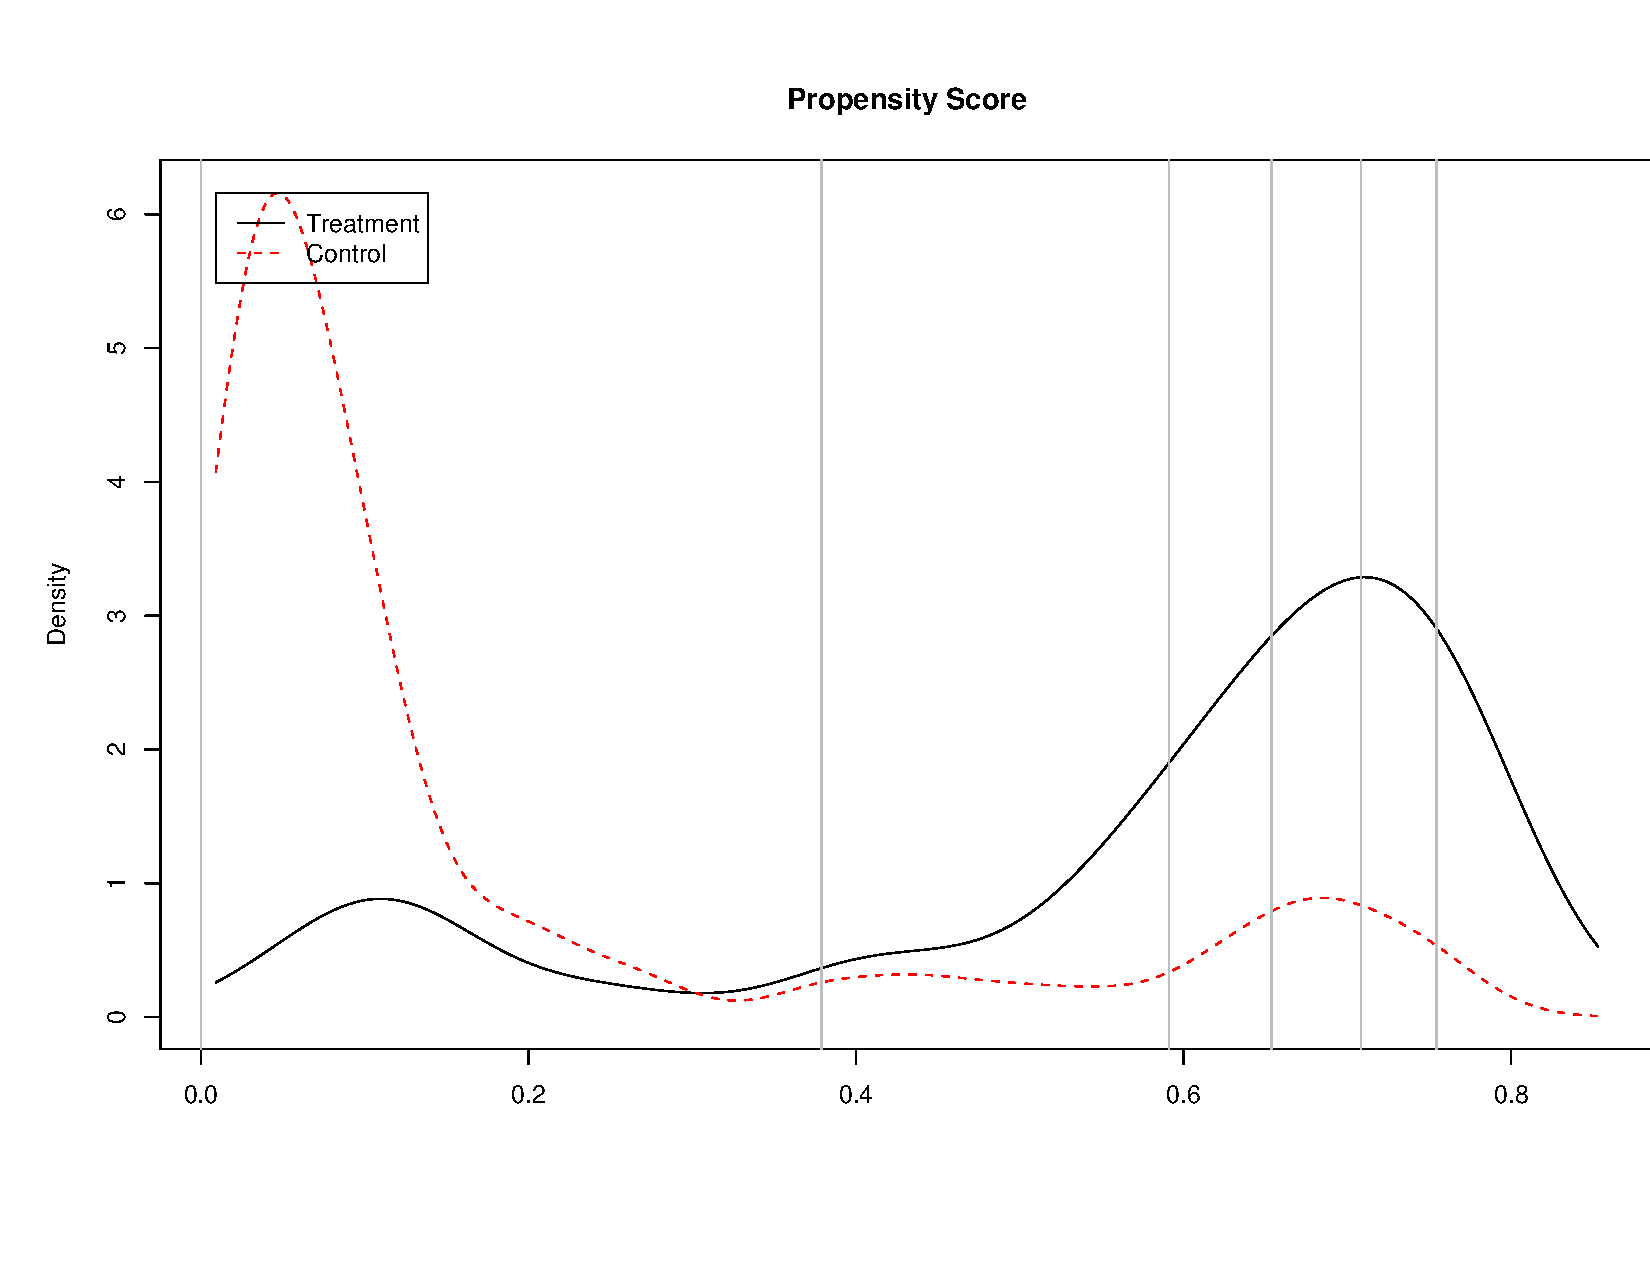
\includegraphics[height=2.85in,angle=0]{figs/subclass1}}
    \rotatebox{270}{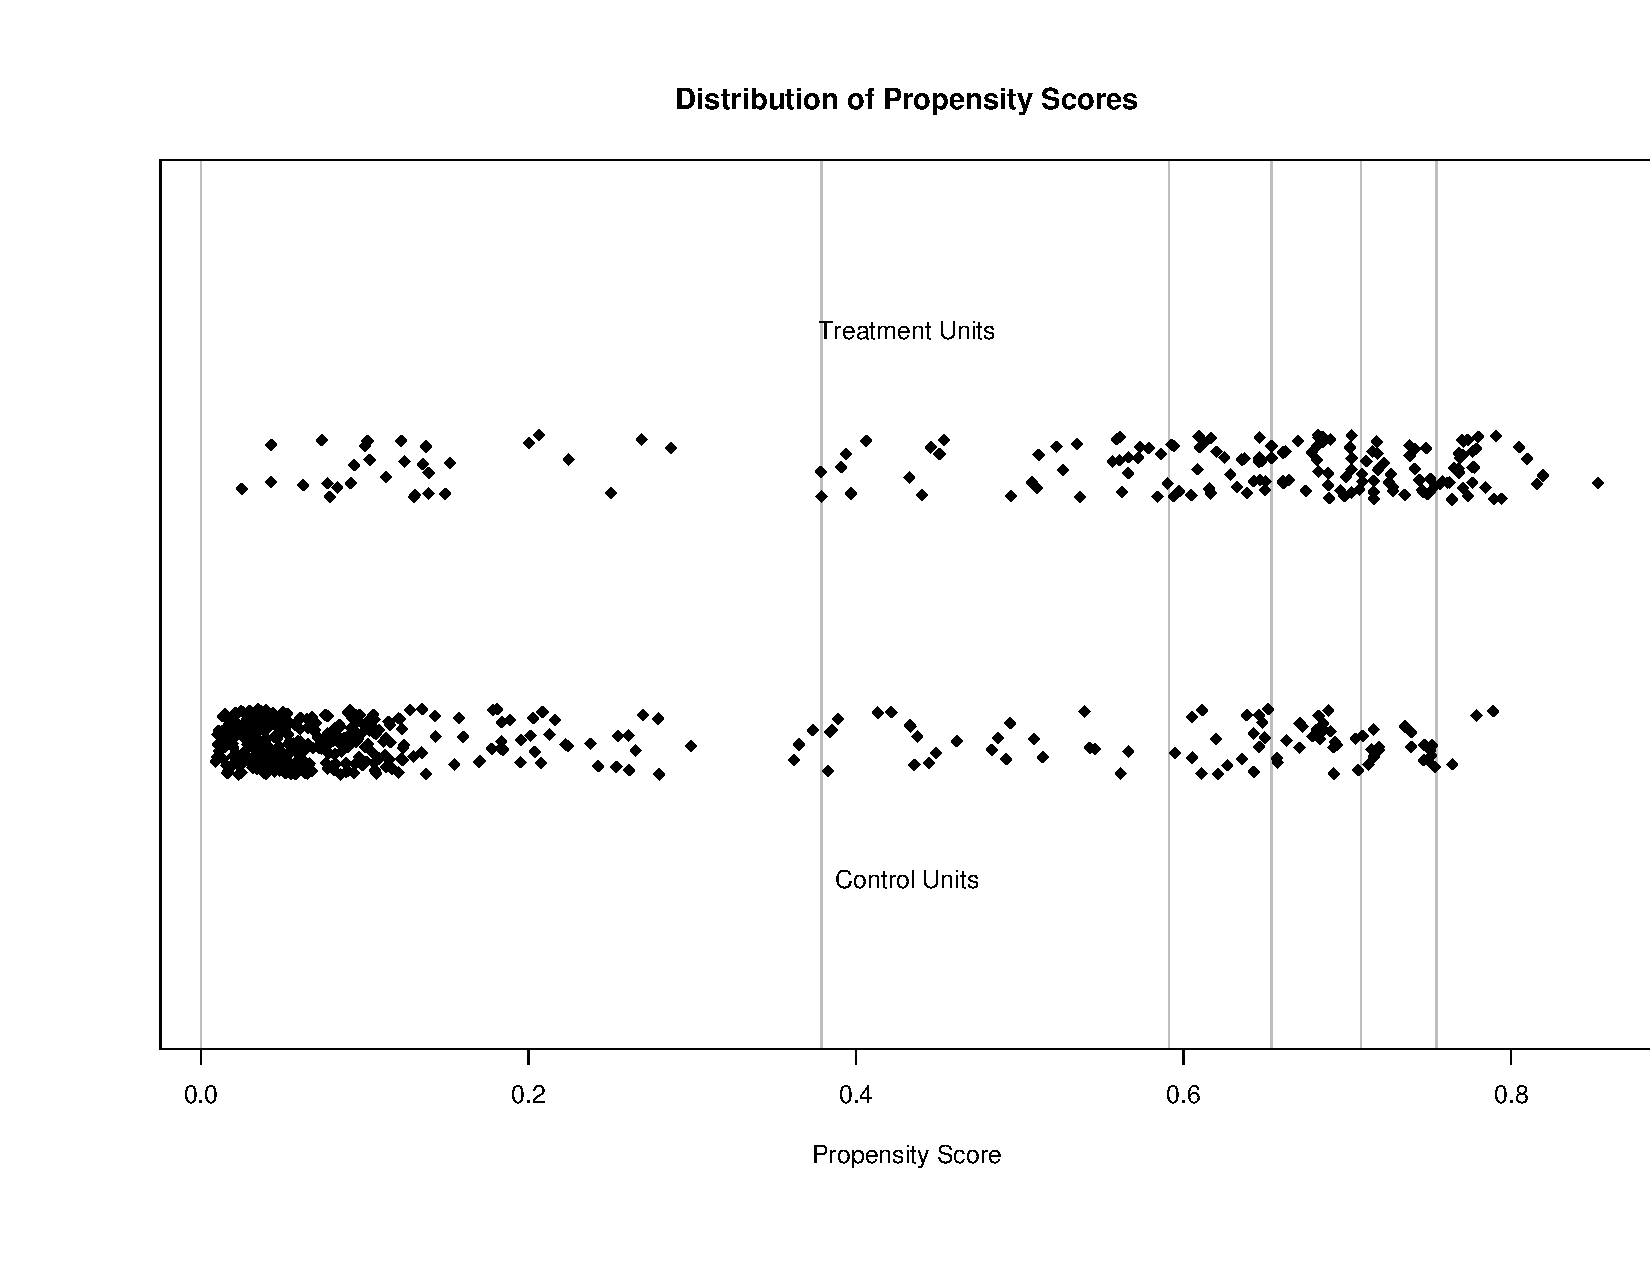
\includegraphics[height=2.85in,angle=0]{figs/subclass2}}
    \rotatebox{270}{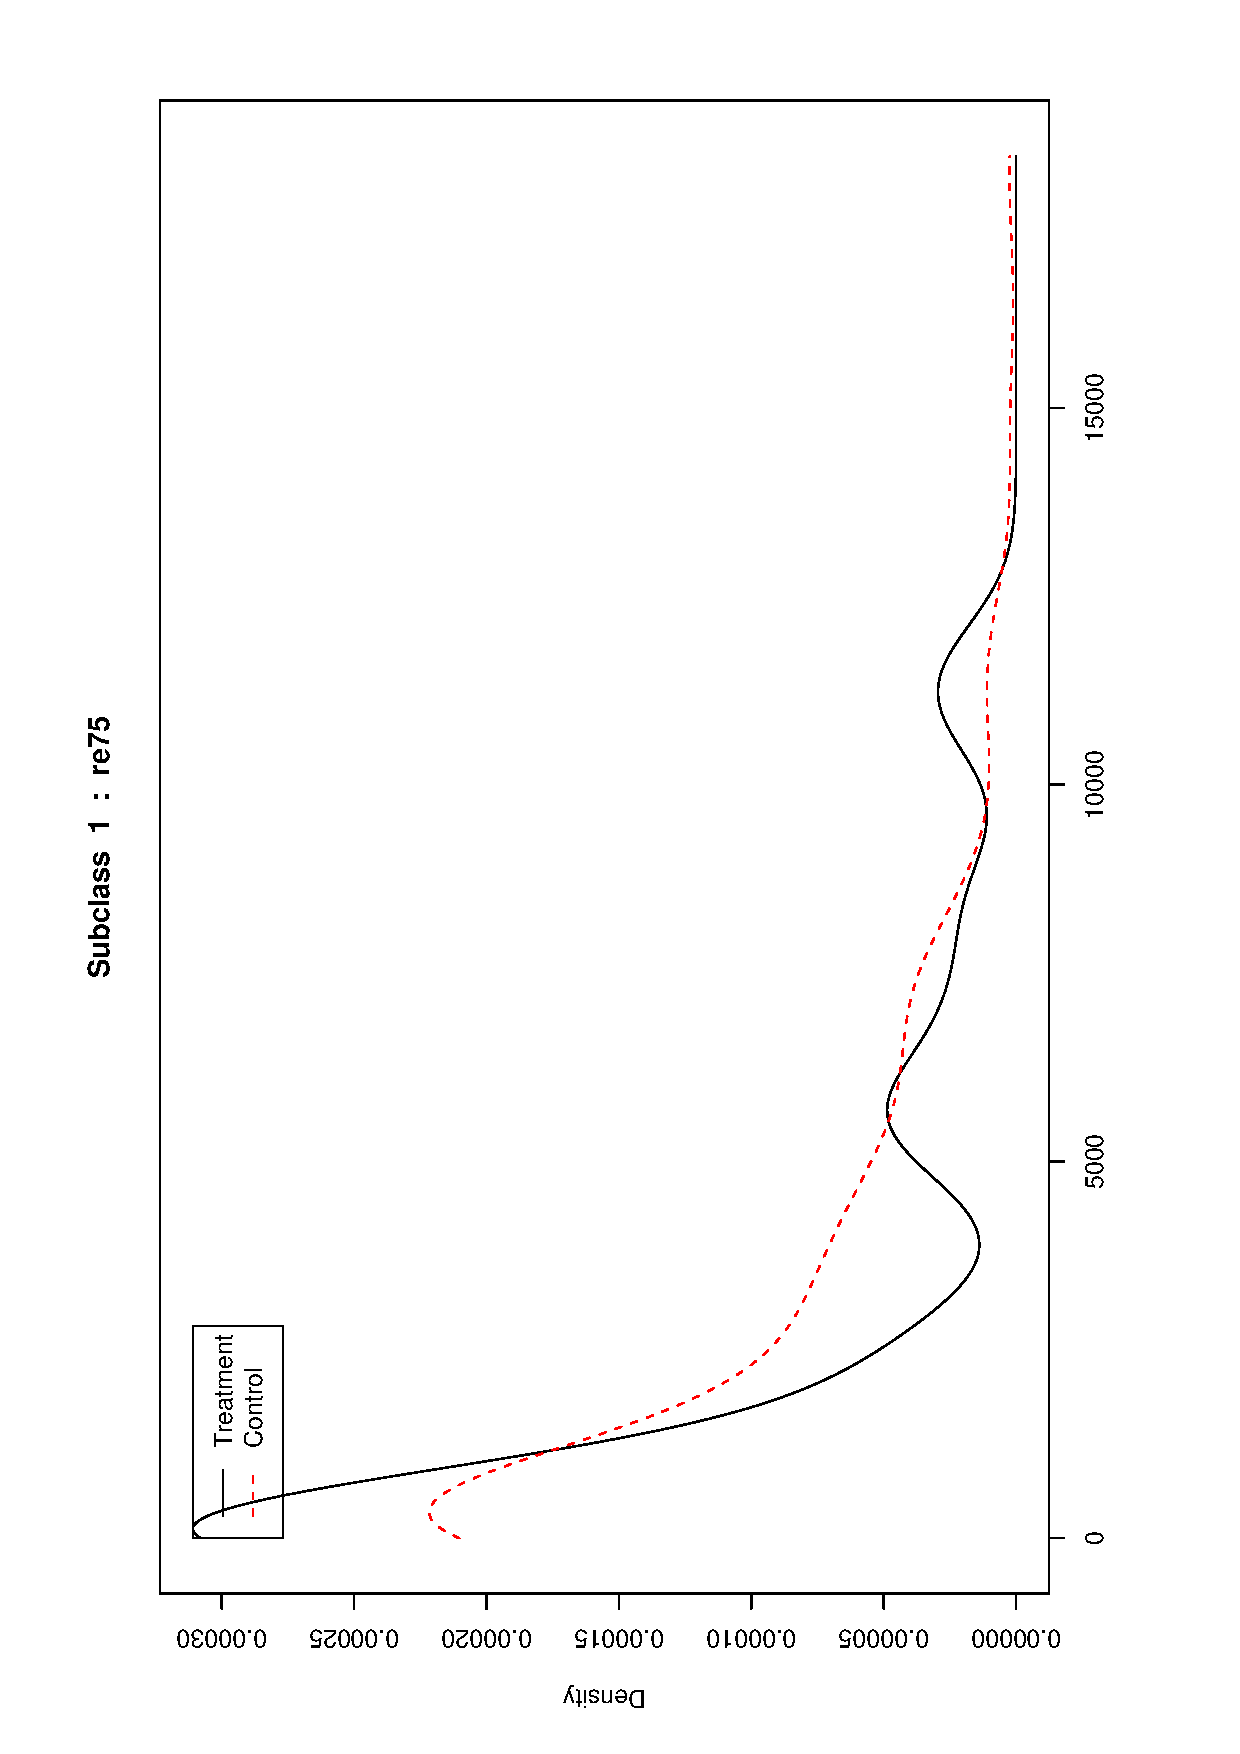
\includegraphics[height=2.85in,angle=0]{figs/subclass3}}
    \rotatebox{270}{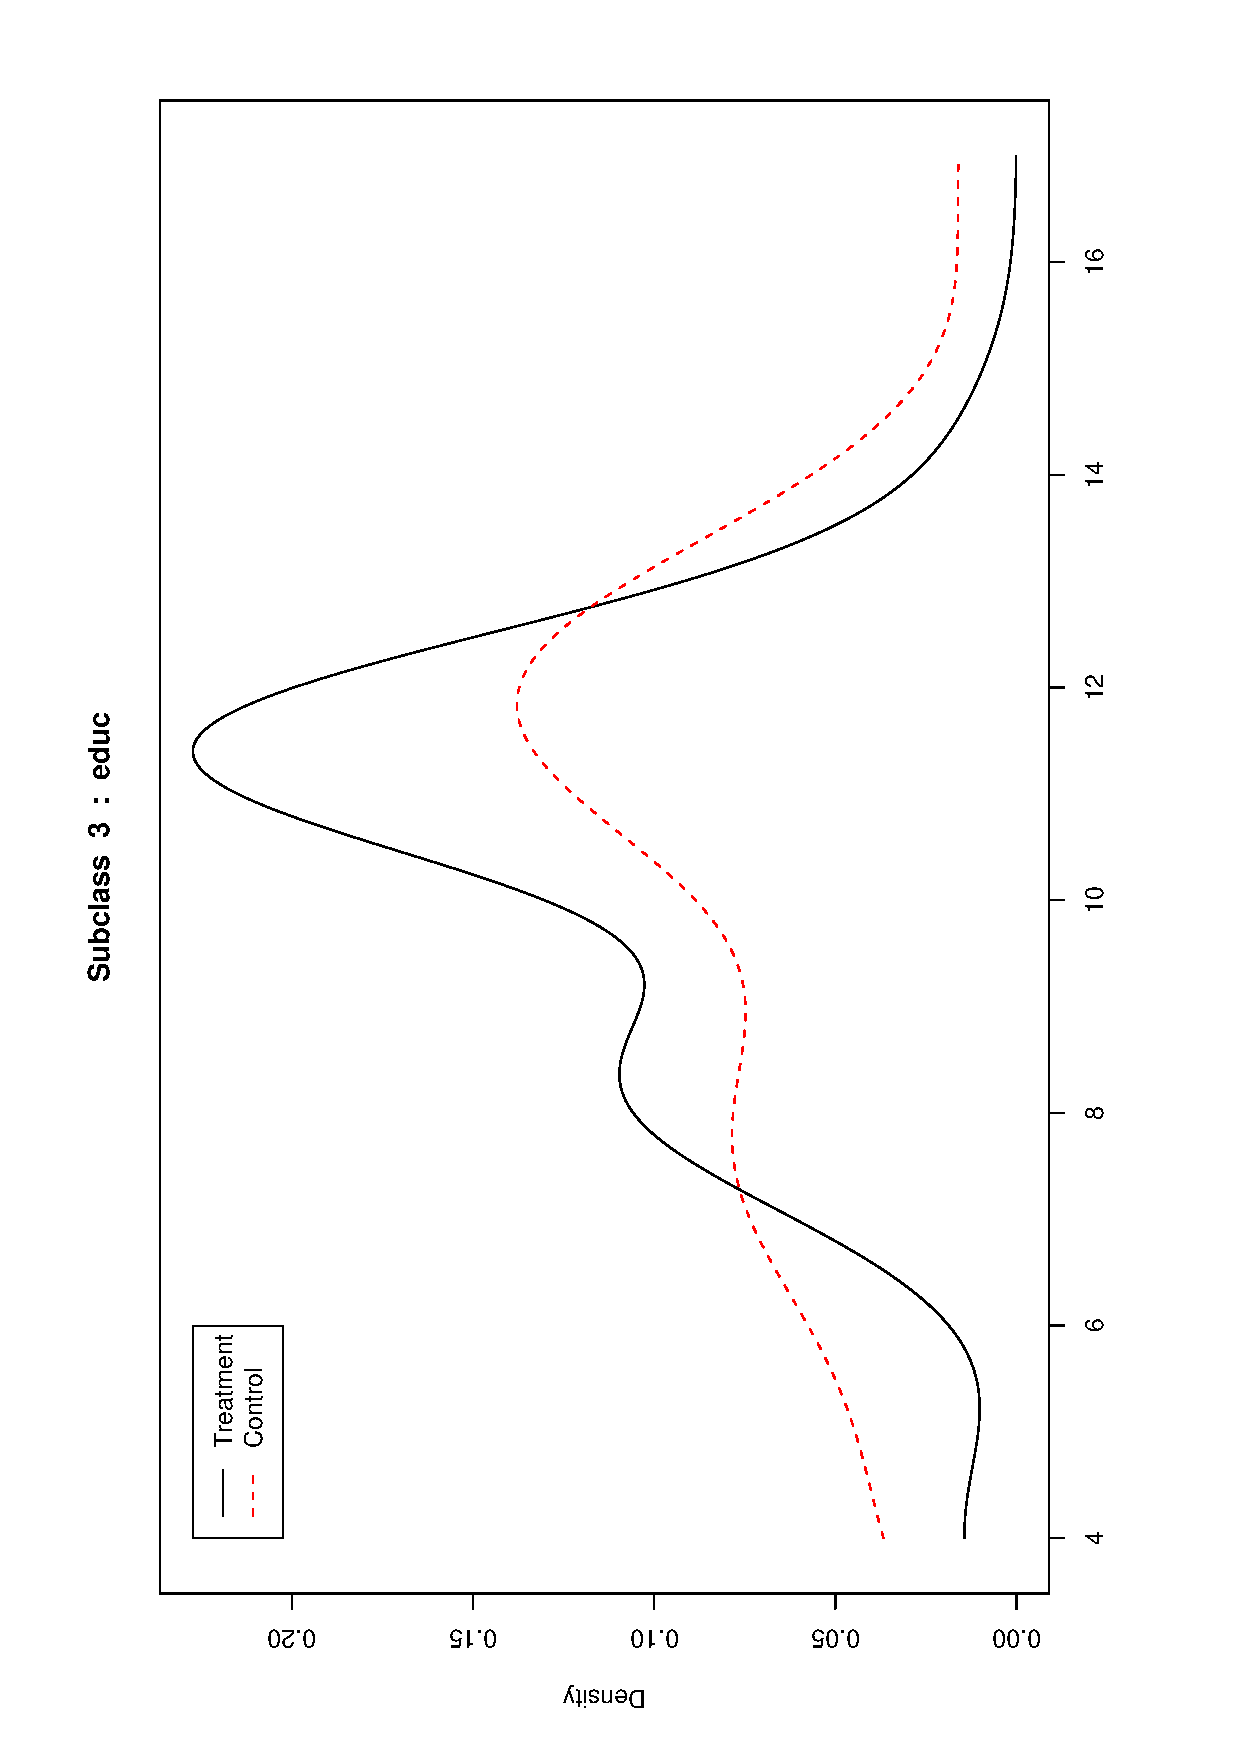
\includegraphics[height=2.85in,angle=0]{figs/subclass4}}
    \hfill
    \caption{Sample interactive diagnostic graphs from \texttt{demo(lalonde)}}
\label{diags}
\end{center}
\end{figure}


\begin{verbatim}
> print(foo2)
 
Assignment model specification:
matchit(formula = treat ~ age + educ + black + hispan + married + nodegree + 
    re74 + re75, data = lalonde, nearest = FALSE, replace = TRUE, subclass = 6)
 
Summary of propensity score for full sample:
 
     Means Treated Means Control     SD T-stat  Bias
Full        0.5774        0.1822 0.2903  20.14 1.794
 
Sample sizes:
 
     Treated Control Total
Full     185     429   614
 
 
Summary of propensity score by subclasses:
 
              Subclass 1 Subclass 2 Subclass 3 Subclass 4 Subclass 5 Subclass 6
Means Treated    0.13761    0.50815    0.62615   0.682281    0.72963    0.78055
Means Control    0.07627    0.46688    0.62923   0.682351    0.73457    0.77741
SD               0.06753    0.06705    0.01897   0.014952    0.01516    0.02037
T-stat           4.20947    2.40592   -0.53366  -0.017308   -1.05718    0.38338
Bias             0.77817    0.60165   -0.15852  -0.004403   -0.34684    0.14896
 
Sample sizes by subclasses:
 
        Subclass 1 Subclass 2 Subclass 3 Subclass 4 Subclass 5 Subclass 6
Treated         31         31         29         32         31         31
Control        346         24         17         21         18          3
Total          377         55         46         53         49         34
\end{verbatim}

\noindent \texttt{q.table} in the {\tt summary} output is also an easy way to provide summaries across
subclasses.  

\subsection{Caliper Matching}

To match within a caliper of 0.25 standard deviations of the
propensity score, use the \texttt{caliper} input:

\begin{verbatim}
> foo <- matchit(treat ~ age + educ + black + hispan + married +
  nodegree + re74 + re75, data=lalonde, caliper=0.25, replace=TRUE)
\end{verbatim}

This restricts the matches to have propensity scores within the
caliper size.  It is usually used in combination with Mahalanobis
matching, as described in Section \ref{mahal}.

If no control units exist within the range of caliper specified, the
treated unit remains unmatched.  In some instances this might result
in very few matched units.  As a result, you may want to increase the
caliper size or match the nearest neighbor when no units within the
caliper are available by specifying \texttt{calclosest=TRUE}.

\subsection{Mahalanobis Metric Matching within Caliper}
\label{mahal}
To match with the Mahalanobis metric within the caliper, specify the
variables on which to compute the metric with the \texttt{mahvars}
input, as well as the \texttt{caliper} input:

\begin{verbatim}
> foo <- matchit(treat ~ age + educ + black + hispan + married +
  nodegree + re74 + re75, data=lalonde, mahvars=c("age","educ"),
  caliper=0.25, replace=TRUE)
\end{verbatim}

\subsection{Mahalanobis Metric Matching}

To perform only Mahalanobis Metric matching, set the
\texttt{caliper=Inf}:

\begin{verbatim}
> foo <- matchit(treat ~ age + educ, data=lalonde,
  mahvars=c("age","educ"), caliper=Inf, replace=TRUE)
\end{verbatim}

\subsection{Assignment Model Specification}

\MatchIt\ permits you to use a wide variety of methods to
estimate the propensity score, including logit (default), probit,
neural networks, generalized additive models, and classification
trees.  These can be specified in the \MatchIt\ call using the
\texttt{model} input.  For example:

\begin{verbatim}
foo1 <- matchit(treat~educ+re74+re75,data=lalonde,model="probit")
foo2 <- matchit(treat~educ+re74+re75,data=lalonde,model="nnet")
foo3 <- matchit(treat~educ+re74+re75,data=lalonde,model="gam")
foo4 <- matchit(treat~educ+re74+re75,data=lalonde,model="cart")
\end{verbatim}

Each use different models to estimate the propensity score.  Before
using any of these techniques, the user is strongly advised to seek
outside resources to understand the theoretical groundings of these
techniques.  For political science articles discussing or implementing
(a) neural networks see \citet{beck99,Zeng99,Zeng00,LagRus02}, (b)
generalized additive models see \citet{BecJac98}, and (c)
classification trees see \citet{RugKimMar03}.  For more general
treatments, see \citet{Bishop95,White92,BreFriOls84}.  See also the
\texttt{glm} library for further control of logit and probit
regressions, the \texttt{nnet} for neural networks, the \texttt{mgcv}
library for generalized additive models, and the \texttt{rpart}
library for classification trees.

\subsection{Using Observation Names}
\label{rnames}

Since the diagnostics often make use of the observation names of the
data frame, you may find it helpful to specify observation names the
data input.  Use the \texttt{row.names} command to achieve this.  For
example, to assign the names ``Dan'', ``Kosuke'', ``Liz'' and ``Gary''
to a data frame with the first four observations in the Lalonde data,
type:

\begin{verbatim}
> test <- lalonde[1:4,]  #taking a lalonde subset
> row.names(test) <- c("Dan","Kosuke","Liz","Gary")  #assigning row names
> print(test)
       treat age educ black hispan married nodegree re74 re75      re78
Dan        1  37   11     1      0       1        1    0    0  9930.046
Kosuke     1  22    9     0      1       0        1    0    0  3595.894
Liz        1  30   12     1      0       0        0    0    0 24909.450
Gary       1  27   11     1      0       0        1    0    0  7506.146
\end{verbatim} 

\subsection{Matching on One Covariate}
\MatchIt\ does not assume a propensity score bounded between 0 and 1.
For example, we could use simply the \texttt{matchdef} command,
documented in Appendix~\ref{reference}, to match nearest neighbors on
one covariate:

\begin{verbatim}
index <- rep(TRUE,nrow(lalonde))   #keeping all units
names(index) <- row.names(lalonde) #assigning obs names
treat <- lalonde$treat
names(treat) <- row.names(lalonde)
re75 <- lalonde$re75
names(re75) <- row.names(lalonde)
foo <- matchdef(treat,index,re75,replace=TRUE)
\end{verbatim}

\subsection{Diagnosing a propensity score model}
\label{pscorespec}
The model specification and diagnostics when estimating propensity
scores are not the standard model diagnostics for logistic regression
or CART, as discussed by \cite{Rubin04}.  With propensity score
estimation, and matching methods more generally, concern is not with
the parameter estimates of the model, but rather with the quality of
the matches.  As discussed by \cite{Greevy04}, because the matching
does not make use of the outcome values, matching can be done multiple
times and the best matched sample chosen without biasing results.
Diagnostics for propensity scores thus involve assessing
specifications and choosing the one that leads to the most balance
between the matched treated and control groups.

\cite{RosRub84a}, \cite{Perkins00}, and \cite{DehWah02} describe
propensity score model fitting strategies that involve examining the
resulting covariate balance in subclasses defined by the propensity
score.  If covariates (or their squares or cross-products) are found
to be imbalanced, those terms are then included in the propensity
score specification, which should improve their balance.  A sample
strategy is described here:

\begin{enumerate}
\item Start with model (for example, logistic regression with
  treatment received as the response variable) with main effects for
  each of the observed covariates.  The propensity scores are the
  predictors of treatment assignment generated from this model.
\item (Optional) Discard control units outside the range of the
  treated group propensity scores, and/or treated units outside the
  range of the control group propensity scores.
\item Form 2 subclass (with propensity scores split at their median),
  do a t-test of the propensity score in the treated and control
  groups in each subclass.  If there is a significant difference,
  split into subclass into 2 subclasses at its median.  Continue this
  process, splitting a subclass if it has a t-statistic greater than
  2.5 and if there are two or more treated and control units in each
  new subclass formed.
\item Within each subclass formed in Step 3, test for equality of
  means of functions of X (e.g., each covariate, each covariate
  squared, 2-way interactions of covariates).  If any t-statistic is
  greater than 2 in any subclass, include that term in the new
  propensity score specification.  (Other, similar rules can be used,
  such as including terms that are significant in more than 1
  subclass).
\item Repeat Steps 1-4 until there are no more (or very few, as few as
  possible) significant t-statistics.  This will imply that within
  each block the treated and control groups are very well balanced.
\end{enumerate}

This method can be implemented in \MatchIt\ in the following way.
First, run a propensity score model with main effects for each of the
covariates, first with just two subclasses, divided at the median
propensity score:

\begin{verbatim}
> match.out1 <- matchit(treat ~ age + married + black + hispan +
                      nodegree + educ + re74 + re75, data=lalonde,                      
                      subclass=c(0, .5, 1))

> summary(match.out1, verbose=F)
\end{verbatim}

The following is an excerpt from the output:

\begin{verbatim}
, , Subclass 1

         means.t.q means.c.q    sd.q    t.q bias.q reduction.q
pscore        0.42      0.26    0.22   5.71   0.55           1
Number       91.00    143.00  234.00 234.00 234.00         234

, , Subclass 2

         means.t.q means.c.q    sd.q    t.q bias.q reduction.q
pscore        0.73      0.71    0.04   2.68   0.06           1
Number       94.00     42.00  136.00 136.00 136.00         136

Problematic covariates:
Subclass  1 :  pscore black hispan
Subclass  2 :  pscore
Number of units discarded:   0

\end{verbatim}

Because the t-statistics of the propensity scores in both subclasses
are greater than 2.5, we divide each block in half, at its median:

\begin{verbatim}
> match.out1 <- matchit(treat ~ age + married + black + hispan +
                      nodegree + educ + re74 + re75, data=lalonde,                      
                      subclass=c(0, .25, .5, .75, 1))

> summary(match.out1, verbose=T)
\end{verbatim}

Because Subclass 4 still has a t-statistic greater than 2.5, we again
divide that subclass in half, leading to five subclasses.  All five
subclasses have t-statistics of the propensity score less than 2.5.
We then run {\tt summary(match.out1, verbose=T)} on that matchit
object, to examine the balance of all of the squares and interactions
of the covariates within each subclass.

\begin{verbatim}
> match.out1 <- matchit(treat ~ age + married + black + hispan +
+                       nodegree + educ + re74 + re75, data=lalonde,
+                       subclass=c(0, .25, .5, .75,.875, 1))
Calculating propensity score...Done
Matching Treated: 10%...20%...30%...40%...50%...60%...70%...80%...90%...100%...Done
Subclassifying...Done
Calculating summary statistics...Done
> summary(match.out1, verbose=T)
\end{verbatim}

We are interested in the ``Problematic covariates".  For subclasses,
this is a list of all covariates, squares, and two-way interactions
that have t-statistics greater than $2$ in any subclass (the default
of $2$ can be changed by specifying the {\texttt sig} option in the
{\texttt summary} command).

\begin{verbatim}
Problematic covariates:
Subclass  1 :  black re74 blackxblack blackxeduc blackxre74
Subclass  2 :  married agexmarried marriedxmarried marriedxblack marriedxnodegree 
               marriedxeduc nodegreexeduc
Subclass  3 :  
Subclass  4 :  agexnodegree
Subclass  5 :  
\end{verbatim}

These ``problematic" covariates are then included in the new
propensity score specification, and the process is repeated.  (Note:
since {\tt black} and {\tt married} are binary covariates, their
squares are just the variables themselves and thus the squares are not
included in the new specification.)

\begin{verbatim}
> match.out2 <- matchit(treat ~ age + educ + married + nodegree + hispan +
                      black + re74 + re75 + I(black*educ) +
                      I(black*re74) + I(age*married) + I(married*black) + 
                      I(married*nodegree) + I(married*educ) +
                      I(nodegree*educ) + I(age*nodegree),
                      data=lalonde, subclass=c(0,.5,1))

> summary(match.out2, verbose=F)
\end{verbatim}

This process leads to three blocks being created  ({\tt subclass=c(0, .25, .5, 1)}).

\begin{verbatim}
> match.out2 <- matchit(treat ~ age + educ + married + nodegree + hispan
                      + black + re74 + re75 + I(educ*black) +
                      I(black*re74) + I(age*married) + I(educ*married)
                      + I(educ*nodegree) + I(married*nodegree) +
                      I(married*black) + I(age*nodegree),
                      data=lalonde, subclass=c(0,.25,.5,1))

> summary(match.out2, verbose=F)
\end{verbatim}

We see that now there are only 2 ``problematic covariates," in just
one subclass.  We use {\tt verbose=F} at this stage so that
we are checking just the balance of the squares and two-way
interactions of the covariates themselves; {\tt verbose=T} here would
give details on the squares and interactions of the interaction
variables, which are generally not of as much interest as the two-way
interactions themselves.  Because good balance has been achieved and the two problematic covariates
are already included, we stop here and use this propensity
score model, with the chosen interactions.

\begin{verbatim}
Problematic covariates:
Subclass  1 :  
Subclass  2 :  re74 I(black * re74)
Subclass  3 :  
\end{verbatim}

This section has provided one example of a diagnostic procedure for
propensity score models.  The details may vary (for example, an option
could be to include only squares and interactions that have a
significant difference in more than one block.  The user could also
identify a different cut-point for the subclasses, or for significance
(as opposed to 2.5 and 2).

\section{Reference}

\subsection{Usage}

The basic syntax to \texttt{matchit} is quite similar to other models in R, such as the
\texttt{lm} or \texttt{glm} models: 

\begin{verbatim}
matchit <- function(formula, data, model="logit", discard=0,
                    reestimate=FALSE, nearest=TRUE, replace=FALSE,
                    m.order=2, ratio=1, caliper=0, calclosest=FALSE,
                    subclass=0, sub.by="treat", mahvars=NULL, exact=FALSE,
                    counter=TRUE,...)
\end{verbatim}

\subsection{Inputs}

\begin{enumerate}
  
\item \textbf{Formula (required).}  \texttt{formula} takes the form of
  {\tt T \~\ X1 + X2}, where {\tt T} is a binary treatment indicator
  and {\tt X1} and {\tt X2} are the pre-treatment covariates, and {\tt
    T}, {\tt X1}, and {\tt X2} are contained in the same data frame.
  The $+$ symbol means ``inclusion'' not ``addition.'' You may also
  include interaction terms in the form of {\tt I(X1*X2)} or squared
  terms in the form of {\tt I(X1 \^\ 2)}.\footnote{The \texttt{I()}
    command ensures that the expression is interpreted as one term.
    If you omit it, the main effects will automatically be included as
    well.}
  
\item \textbf{Dataframe (required).}  \texttt{data} specifies the data
  frame containing the variables called in the formula.  You may find
  it helpful for the diagnostics to specify observation names in the
  data frame.  To do this, see Section~\ref{rnames}.  Please note that
  the dataframe should not include variables with the names
  \texttt{psclass}, \texttt{psweights}, and \texttt{pscore}, as these
  are expressly reserved in the output dataframe for \MatchIt. 
  
\item \textbf{Assignment Model.}The assignment model estimation may be
  changed by \texttt{model}, which specifies the method used to
  estimate the propensity score:
  \begin{enumerate}
  \item \texttt{logit}, the default method, implements a logistic
    regression.  See {\tt help(glm)} for more options.
  \item \texttt{probit} implements a probit regression.  See {\tt
      help(glm)} for more options.
  \item \texttt{nnet} implements a neural network in the \texttt{nnet}
    library, with a default size of 3.  See {\tt help(nnet)} for more
    options.
  \item \texttt{GAM} implements a generalized additive model as in the
    \texttt{mgcv} library.  See {\tt help(gam)} for more options.
  \item \texttt{cart} implements a classification tree as in the
    \texttt{rpart} library.  See {\tt help(rpart)} for more options.
  \end{enumerate}
  
\item \textbf{Discarding.} \texttt{discard} specifies whether to
  discard units that fall outside some measure of support of the
  distance score:
  \begin{itemize}
  \item default=0 keeps all units.  Use this option when the units to
    be matched are substantially similar, such as in the case of
    matching treatment and control units from a field experiment that
    was close to (but not fully) randomized (e.g., \citealt{Imai03}).
    (Other reasons for keeping all units may be that subclassification
    on all units is desired or that caliper matching will naturally
    restrict the donor pool.)
  \item 1 keeps all units with common support on the distance measure.
    Use this option when the units to be matched are substantially
    different (when there is a large degree of non-overlapping
    support on the distance score), such as in the case of measuring
    the effect of democracy on economic growth (e.g.,
    \citealt{KinZen03b}).
  \item 2 discards only control units outside the support of the
    distance measure of the treated units.  Use this option when the
    average treatment effect on the treated is of most interest and
    when unwilling to discard non-overlapping treatment units, such as
    possibly in the case of the effect of job training on those
    individuals that actually participated in a job evaluation program
    (e.g., \citealt{HecIchTod98}) or a drug study where interest is in all patients treated with the drug.
  \item 3 discards only treated units outside the support of the
    distance measure of the control units.  Use this option when the
    average treatment effect on the control units is of most interest
    and when unwilling to discard control units.
  \end{itemize}
  
\item \textbf{Reestimation.} \texttt{reestimate} specifies whether the
  propensity score model should be re-estimated after units are
  discarded, default=FALSE.  This may be desirable for efficiency
  reasons, especially if many units were not matched so that the
  matched samples are quite different from the original samples.

\item \textbf{Advanced Matching}
  \begin{itemize}
  \item \texttt{nearest} is a logical scalar which specifies whether
    to perform nearest-neighbor matching, default=TRUE.  Using
    \texttt{nearest=FALSE} can provide a more efficient way to
    perform only subclassification. 
  \item \texttt{m.order}  specifies the order in which to match
    treatment units with control units:
    \begin{itemize}
    \item (2) indicates matching from highest propensity scores to
      lowest (default).
    \item (3) indicates matching from lowest propensity scores to
      highest.
    \item (4) indicates matching in random order.
    \item (1) is a placeholder for optimal matching that is yet to be
      developed.
    \end{itemize}
  \item \texttt{caliper} specifies the standard deviations of 
    the propensity score within which to draw control units,
    default=0.  If \texttt{caliper!=0}: 
    \begin{itemize} 
    \item \texttt{calclosest} specifies whether to take the nearest
      available match if no matches are available within
      \texttt{caliper} (default=FALSE).
    \item \texttt{mahvars} specifies variables on which to perform
      Mahalanobis-metric matching within each caliper, default=NULL.
      Variables should be entered as a vector of variable names
      \texttt{mahvars=c("X1","X2")} that are names of variables in
      \texttt{data}.
    \end{itemize}
  \end{itemize}
  
\item \textbf{Replacement matching.} \texttt{replace} is a logical
  vector which specifies whether to match with replacement (i.e.,
  whether each control unit can be matched to more than one treated
  unit), default=FALSE.  Use this to reduce bias when the ratio of
  control units that are comparable to the treated units is small and
  when pre-treatment covariates between treatment and control units
  diverge substantially.
  
\item \textbf{Ratio Matching.}  \texttt{ratio} specifies the number of
  control units to be matched to each treatment unit, default=1.  To
  increase efficiency of the estimand when there is a large number of
  comparable control units available, use larger integer values. If
  matching is done without replacement and there are fewer control
  units than ratio times the number of eligible treated units (i.e.
  there are not enough control units for the specified method), then
  the higher ratios will have \texttt{NA} in place of the matching
  unit number.

\item \textbf{Subclassification}
  Subclassification options allow the user to subclassify units along
  the propensity score:
  \begin{itemize}
  \item \texttt{subclass} is either (1) a scalar, specifying the
    number of subclasses, or (2) a vector of probabilities bounded
    between 0 and 1, to create quantiles based on \texttt{subtype},
    where the value of 0 (default) indicates no subclassification.
  \item If \texttt{subclass!=0}, \texttt{sub.by} specifies by what
    criteria to subclassify: \texttt{``treat''} indicates by the
    number of treatment units (default), \texttt{``control''}
    indicates by the number of control units, and \texttt{``all''}
    indicates by the total number of units.
  \end{itemize}
  The subclass options create quantiles corresponding to the given
  probabilities from \texttt{subclass}, using the \texttt{quantile}
  command on the propensity scores of the \texttt{sub.by} units.
  
\item \textbf{Exact Matching.}  \texttt{exact} specifies whether exact
  matching should be done.  \texttt{FALSE} (default) indicates no
  exact matching.  \texttt{TRUE} indicates exact matching on all
  variables in the assignment model of the \texttt{formula} (i.e., the
  propensity score will never be generated).  A vector of variable
  names indicates separate variables on which to exact match, in
  combination with matching on the propensity score.  This option will
  not be different from \texttt{exact=TRUE}, unless the list differs
  from the variables in the formula.\footnote{For example,
    \texttt{matchit(T \~\ X1 + X2, data, exact=TRUE)} is equivalent to
    \texttt{matchit(T \~\ X1, data, exact=cbind(X1,X2))}.  But
    \texttt{matchit(T \~\ X1 + X2, data, exact=X1)} will match units
    exactly only on \texttt{X1} and perform nearest neighbor matching
    on the propensity score which uses \texttt{X1} and \texttt{X2}.}
  Variables should be entered as a vector of names
  \texttt{exact=c("X1","X2")} that refer to variable names in
  \texttt{data}.
  
\item \textbf{Counter.} \texttt{counter} specifies whether a counter
  indicating the progress of the matching is displayed.  \texttt{TRUE}
  (default) means that this counter will be displayed, \texttt{FALSE}
  means that it will not be displayed.

\end{enumerate}
  
\subsection{Output}

The following are the outputs of each \texttt{matchit} object; if
outputs are not applicable for the original \texttt{matchit} call,
they are returned as \texttt{NA}:

\begin{enumerate}
  
\item \texttt{call} provides the original \MatchIt\ call.
 
\item \texttt{formula} shows the formula used to specify the
  propensity score model.
  
\item \texttt{match.matrix} is an $n_1$ by \texttt{ratio} data frame,
  where:

  \begin{itemize}
  \item the row names, \texttt{row.names(match.matrix)}, store the
    names of the treatment units, which come from the data frame
    specified in \texttt{data} (to learn how to do this, see
    Section~\ref{rnames}),
  \item each column stores the name(s) of the control unit(s) matched
    to the treatment unit of that row (e.g., when the \texttt{ratio}
    input is specified as 3, the three columns of
    \texttt{match.matrix} represent the three control units matched to
    one treatment unit),
   \item \texttt{NA} indicates that the treatment unit was not
     matched.  
   \end{itemize}
   
 \item \texttt{in.sample} is a vector of length $n$ that displays
   whether the units were eligible for matching due to discarding due
   to common support restrictions.  If unit $i$ was discarded,
   \texttt{in.sample[i]=FALSE}, and if unit $i$ was not discarded
   \texttt{in.sample[i]=TRUE}.
   
 \item \texttt{matched} is a vector of length $n$ that displays
   whether each unit was matched.  \texttt{matched==TRUE} means that
   unit was matched, whereas \texttt{matched==FALSE} means it was not.
   
 \item \texttt{psweights} is a vector of length $n$ that provides the
   weights assigned to each unit in the matching process.  Unmatched
   units have weights equal to $0$. Matched treated units have weight
   $1$.  Each matched control unit has weight proportional to the
   number of times it was matched.  The sum of the control weights is
   equal to the number of uniquely matched control units.
   
 \item \texttt{psclass} contains the subclass index in an ordinal
   scale from 1 to the total number of subclasses as specified in
   \texttt{subclass}; a higher subclass refers to a higher propensity
   score.  Unmatched units have \texttt{psclass=0}.
   
 \item \texttt{q.cut} gives the subclass cut-points.
   
 \item \texttt{assign.model} stores the output of the assignment
   model.  For example:
  
  \begin{footnotesize}
\begin{verbatim}
> foo <- matchit(treat~ age + educ + black + hispan + married +
      nodegree + re74 + re75,data=lalonde)
> print(foo$assign.model)

Call:  glm(formula = treat ~ age + educ + black + hispan + married +
      nodegree + re74 + re75, family = binomial, data = lalonde) 

Coefficients:
(Intercept)          age         educ        black       hispan      married  
  7.077e-01   -8.696e-02    1.257e-01    1.690e+00    9.011e-01   -1.484e+00  
   nodegree         re74         re75  
  1.171e+00   -7.810e-05    1.957e-05  

Degrees of Freedom: 312 Total (i.e. Null);  304 Residual
Null Deviance:      423.5 
Residual Deviance: 253.1        AIC: 271.1 
\end{verbatim}
\end{footnotesize}

\item \texttt{data} is a data frame that contains the original data
  set in the \MatchIt\ call, as well as three additional variables:
  \texttt{psclass}, \texttt{psweights}, and \texttt{pscore}
  (\texttt{pscore} is a vector of $n$ length that contains the
  estimated propensity scores for all units (i.e., the probability of
  treatment assignment conditional on the covariates)).
  
\item \texttt{treat} stores the treatment indicator from \texttt{data}
  (the left-hand side of the assignment model).
  
\item \texttt{covariates} stores the covariates used in the right-hand
  side of the assignment model.
\end{enumerate}

\subsection{Print, Plot and Summary Commands}
\subsubsection{Print}
The \texttt{print} command returns (when applicable):
\begin{enumerate}
\item The original assignment model call.
\item Summary statistics of the propensity score for full and matched
  samples.
\item Summary statistics of the propensity score for each subclass.
\item Sample sizes for full and matched samples (full and by subclass).
\end{enumerate}

\subsubsection{Summary}
\label{cmd:sum}
The \texttt{summary} command returns more information about the
\MatchIt\ model.  Optional inputs are:

\begin{enumerate}
\item \texttt{sig}, which specifies the size of the t-statistic for a
  covariate to be declared ``problematic'' (default=2).
  
\item \texttt{verbose}, which is an option to show calculate summary
  statistics in \texttt{sum.all} and \texttt{sum.matched} for all
  covariates, their squares, and interactions when
  \texttt{verbose=TRUE} and only the covariates themselves when
  \texttt{verbose=FALSE} (default).
\end{enumerate}

The \texttt{summary} call returns, when applicable:

\begin{enumerate}
\item The original assignment model call.
\item \texttt{sum.all} is a data frame which contains variable names
  and interactions down the row names, and summary statistics on
  \emph{all observations} in each of the columns.  The columns in
  \texttt{sum.all} contain:
  \begin{itemize}
  \item means of all covariates $X$ for treated and control units,
    where \texttt{Means Treated}$= \mu_{X|T=1} = \frac{1}{n_1}
    \sum_{T=1} X_i$ and \texttt{Means Control}$= \mu_{X|T=0} =
    \frac{1}{n_0} \sum_{T=0} X_i$,
  \item standard deviations for all covariates $X$, where
    \texttt{SD}$= s_X = \sqrt{\frac{1}{n-1} \sum_{i} (X_i -
      \overline{X})^2}$,
  \item t-statistics from means tests of all covariates $X$,
    \texttt{T-stat},\footnote{Note that the t-tests do not assume
      constant variance across treatment and control groups, using a
      pooled estimate of the standard deviation.  For this reason, the
      t-statistics do not correspond to the overall standard
      deviations reported in \texttt{SD}.  For more information, see
      \texttt{help(t.test)}.} and
  \item matchit bias statistics \texttt{Bias}$=\frac{\mu_{X|T=1} -
      \mu_{X|T=0}}{s_{x|T=1}}$, \\ where $s_{x|T=1} =
    \sqrt{\frac{1}{n_1-1} \sum_{T=1} ( (X_i|T_i=1) - \mu_{X|T=1})}$.
  \end{itemize}
  
\item \texttt{sum.matched} is a data frame which contains variable
  names down the row names, and summary statistics on only the
  \emph{matched observations} in each of the columns.  Specifically,
  the columns in \texttt{sum.matched} contains:
  \begin{itemize}
  \item weighted means for matched treatment units of all covariates
    $X$ and their interactions, where \texttt{Means Treated}$=
    \mu_{wX|T=1} = \frac{1}{n_1} \sum_{T=1} w_iX_i$ and \texttt{Means
      Control}$=\mu_{wX|T=0} = \frac{1}{n_0} \sum_{T=0} w_iX_i$,
  \item weighted standard deviations for all covariates $X$ and their
    interactions of matched units, where \texttt{SD} $= s_{wX} =
    \sqrt{\frac{1}{n} \sum_{i} (w_iX_i - \overline{wX})^2}$,
  \item t-statistics (weighted by {\texttt psweights}) from means
    tests of all covariates $X$ and their interactions
    \texttt{T-stat},\footnote{Note that the weighted t-tests do not
      assume constant variance across treatment and control groups,
      using a pooled estimate of the standard deviation.  For this
      reason, the weighted t-statistics do not correspond to the
      overall standard deviations reported in \texttt{SD}.  For more
      information, see \texttt{help(t.test)}.}
  \item balance bias statistics \texttt{Bias}$=\frac{\mu_{wX|T=1} -
      \mu_{wX|T=0}}{s_{x|T=1}}$, and
  \item a column indicating whether there was a reduction in the
    absolute balance bias compared to all units (1 indicates a
    reduction, and 0 indicates no reduction),
  \end{itemize}
  
  where $w$ represents the vector of \texttt{psweights}.  The last row
  of \texttt{sum.matched} contains the number of matched treated
  units, the number of matched control units, and the total number of
  matched units.
  
\item Problematic covariates that remain imbalanced in the matched
  sample or in each subclass.  A variable is listed when the absolute
  value of the t-statistic in the matched sample exceeds \texttt{sig}
  (default=2).
  
\item \texttt{xn} gives the sample sizes in the full and matched
  samples.
  
\item \texttt{q.table} is an array that contains the same information
  as \texttt{sum.all} and \texttt{sum.matched} by subclass.
  
\item \texttt{qn} gives the sample sizes in the full and matched
  samples, by subclass.
\item \texttt{match.matrix} from the {\texttt matchit} output.
\item \texttt{psclass} from the {\texttt matchit} output.
\item \texttt{in.sample} from the {\texttt matchit} output.
\end{enumerate}

\subsubsection{Plot}
The \texttt{plot} command allows the user to check the distributions
of all covariates in the assignment model, squares, and interactions,
within all subclasses.  The graphs present:
\begin{enumerate}
\item Density estimate graphs of the propensity score of treated and
  control units in the full and matched samples.
\item Jitter plots of the propensity score for treated and control
  units.
\item Density estimate graphs of any covariates.
\item Density estimate graphs of any covariates by subclass.
\end{enumerate}

\section{Analysis}

Once the matching is complete, the \MatchIt\ object can be used with
any other analysis procedure; \MatchIt\ is designed to make those
analysis procedures less dependent on the modeling assumptions and
thus work better.  Thus, any analysis that the user was going to do on
the original data sets can be done on the matched data sets.

To obtain the matched data sets, use {\tt match.data(match.out)},
where {\tt match.out} is a \MatchIt\ object.
{\tt match.data(match.out, "treat")} gives just the matched treated units, and \\
{\tt match.data(match.out, "control")} gives just the matched control
units.

Here we describe two possible analysis methods to use with \MatchIt.

\subsection{Neyman function}

{\tt neyman} is a \MatchIt\ function which calculates a simple
difference in means and corresponding variance estimate.  The
estimated treatment effect is:
\begin{equation}
\label{ate} 
\widehat{ate} = \overline{y}_{mt}^w-\overline{y}_{mc}^w,
\end{equation}
where $\overline{y}_a^w$ is the weighted mean of the outcome in group
$a$ ($mt$ refers to the matched treated group, and $mc$ refers to the
matched control group).  The weighted mean is calculated as:
$$\overline{y}_a^w = \frac{\sum_{i=1}^n w_i y_i}{\sum_{i=1}^n w_i},$$
where $y_i$ is the outcome and $w_i$ is the weight for individual $i$
({\tt psweights} from the \MatchIt\ object).

The estimated variance of the estimated treatment effect in Equation
\eqref{ate} is:
\begin{equation}
\label{estvar}
\widehat{{\rm var}}(\widehat{ate}) = \frac{s_{mt}^2}{\sum_{i=1}^{n_1} w_i} + \frac{s_{mc}^2}{\sum_{i=1}^{n_0} w_i},
\end{equation}
where $s_a^2$ is the weighted variance of the outcome in group $a$,
and $n_1$ and $n_0$ are the sizes of the matched treated and control
groups, respectively.  The weighted variance in group $a$ is
calculated as:
$$s^2_{a} = \frac{\sum_{i=1}^{n_a} w_i
  (y-\overline{y}_a^w)^2}{(\sum_{i=1}^{n_a} w_i) - 1}.$$

Neyman ??? showed that the variance estimate in Equation
\eqref{estvar} is unbiased for the true variance when the treatment
effect is additive and constant for all individuals ($Y_i(1)-Y_i(0)=c$
for all $i$) and overestimates the true variance when the effect is
non-additive.

If subclasses were formed using \MatchIt, then the Neyman function
will also compute within-subclass estimates and a weighted average
across the subclasses.  The weighted average will be weighted by the
{\tt sub.by} option in the \MatchIt\ call (the number of treated units,
the number of control units, or the total number of units in each
subclass).  If interest is in estimating the average treatment effect
for the treated, the number of treated units in each subclass should
be used for the subclassification and weighting.  Subclasses with
fewer than two treated or control units are not used in the estimation
of the average treatment effect and its variance; they are given a
weight of zero.

Using the Neyman function, it is also possible to estimate the
variance of the estimated treatment effect using the bootstrap.  With
that option, the user specifies a number of bootstrap samples.  An
estimated treatment effect is calculated for each bootstrap sample,
and the variance of the estimated treatment effects is given by the
sample variance of the bootstrap estimates.  

The format of {\tt neyman} is:

\begin{verbatim}
> neyman(Y, object, bootstrap=NULL, counter=TRUE)
\end{verbatim}

{\tt Y} is the outcome of interest, {\tt object} is the \MatchIt\ 
object, {\tt bootstrap} (optionally) specifies how many bootstrap
replications to use in calculating the variance, and {\tt counter}
gives an option of not having a counter indicate what proportion of
the bootstrap samples have been completed.  The output of {\tt neyman}
is the estimated treatment effect and its estimated standard
deviation.  If {\tt match.out} is subclassified, the subclass
estimates can be obtained by using the {\tt summary} command on the
{\tt neyman} output object.  Examples are provided below, which can be
run using {\tt demo(analysis)}.

\subsubsection{Simple Neyman calculation}
Here we provide a simple example of the use of the {\tt neyman} function.

\begin{verbatim}
> match.out1 <- matchit(treat ~ age + educ + black + hispan + nodegree +
+                       married + re74 + re75, data = lalonde)
> neyman.out <- neyman(re78, match.out1)
> print(neyman.out)
 
 Average Treatment Effect:
  
ATE  SD
908 731
 
> summary(neyman.out)
 
 Average Treatment Effect:
        Estimate Std. Error z value Pr(>|z|)
Overall      908        731    1.24     0.21
 
 
 Sample Sizes:
        Ntrt Ncont
Overall  185   185
\end{verbatim}

Thus, the treatment appears to increase real earnings in 1978 by an
average of $\$908$ for individuals in the treated group, with standard
error $731$.

\subsubsection{Neyman within subclasses}
The {\tt neyman} function can also be used with subclassification.  By
default, {\tt sub.by="treated"} and thus the subclassification and
subclass weights are done using the number of treated individuals.
Thus, the subclasses below have approximately equal numbers of treated
units in each subclass.

\begin{verbatim}
> match.out1s <- matchit(treat ~ age + educ + black + hispan + nodegree
                 + married + re74 + re75, data = lalonde, subclass=4)
> neyman.outs <- neyman(re78, match.out1s)
> print(neyman.outs)
 
 Average Treatment Effect:
  
 ATE   SD
1232  840
 
> summary(neyman.outs)
 
 Average Treatment Effect:
           Estimate Std. Error z value Pr(>|z|)
Overall        1232        840    1.47     0.14
Subclass 1     1312       1212    1.08     0.28
Subclass 2     2310       1532    1.51     0.13
Subclass 3     1768       1550    1.14     0.25
Subclass 4     -413       2228   -0.19     0.85
 
 
 Sample Sizes:
           Ntrt Ncont
Overall     185   185
Subclass 1   46   121
Subclass 2   45    22
Subclass 3   47    28
Subclass 4   47    14
\end{verbatim}

\subsubsection{Neyman with exact matching}
The {\tt neyman} function can also be used with exact matching on
covariates.  For exact matching, an overall estimated treatment effect
is calculated, using the {\tt psweights} as weights.

\begin{verbatim}
> match.out1e <- matchit(treat ~ black + hispan, data = lalonde, exact=TRUE)
> neyman.oute <- neyman(re78, match.out1e)
> print(neyman.oute)
 
 Average Treatment Effect:
  
 ATE   SD
1093  657
 
> summary(neyman.oute)
 
 Average Treatment Effect:
        Estimate Std. Error z value Pr(>|z|)
Overall     1093        657    1.66    0.096 .
---
Signif. codes:  0 `***' 0.001 `**' 0.01 `*' 0.05 `.' 0.1 ` ' 1
 
 
 Sample Sizes:
        Ntrt Ncont
Overall  185   429
\end{verbatim}

\subsection{Linear regression on matched samples}
Linear regression is a common method for estimating causal effects.
\MatchIt\ helps ensure that the regression is done using treated and
control groups with similar covariate distributions, thus reducing
reliance on the linearity assumption and extrapolation.  The ordinary
least squares regression can be fit to the matched data, using the
{\tt match.data} function:

\begin{verbatim}
> lm.1 <- lm(re78 ~ treat + pscore, data=match.data(match.out1))
> summary(lm.1)$coef[2,]
  Estimate Std. Error    t value   Pr(>|t|)
 1340.0095   801.4961     1.6719     0.0954


\end{verbatim}

\subsection{Using Zelig for analysis}
Zelig is an easy-to-use R program estimates a variety of statistical
models, gives easily interpretable results by simulating quantities of
interest, and provides numerical and graphical summaries.  The package
along with the complete documentation is available at
\href{http://gking.harvard.edu/zelig/}{http://gking.harvard.edu/zelig/}.
\MatchIt\ and Zelig can be easily used together to enable estimation
of causal effects in very general settings.

Here we provide a few examples of how to use Zelig with \MatchIt\ 
objects.  The general framework is that of imputing the missing
potential outcomes.  For example, for the treated group, the outcomes
under control, $Y(0)$, are missing, whereas the outcomes under
treatment, $Y(1)$, are observed.  We impute these missing outcomes in
the following manner. First, we estimate a model for $Y(0)$ using the
observed outcomes of the matched control units. Then, given this
model, the missing outcome $Y(0)$ are imputed for the matched treated
units. Once those potential outcomes are imputed, the estimation of
individual $i$'s treatment effect, $Y_i(1)-\widehat{Y_i(0)}$, is
straightforward. The average treatment effect for any subpopulation,
e.g., the average treatment effect for the treated individuals, can be
similarly calculated. An advantage of this simulation approach is that
the uncertainty estimates such as standard errors are obtained easily.

\subsubsection{Basic analysis with Zelig}
A few steps are required to obtain estimates of the average treatment
effect.

First, using Zelig, fit a model of the outcome with the covariates or
propensity score as predictors, using just the matched control group.
Here we use a linear model ({\tt "lm"}), however Zelig can support a
wide range of models.  For more details, see the Zelig documentation
at \href{gking.harvard.edu/zelig}{gking.harvard.edu/zelig}.

\begin{verbatim}
> library(Zelig)
> match.out1 <- matchit(treat ~ age + educ + black + hispan + nodegree +
                      married + re74 + re75, data = lalonde)
> z.out1 <- zelig(re78 ~ pscore, data = match.data(match.out1,
                                 "control"), model = "ls")
\end{verbatim}

Next, set the $x$ variables to the covariates observed in the matched
treated units:
\begin{verbatim}
> x.out1 <- setx(z.out1, data = match.data(match.out1, "treat"), cond =
               TRUE)
\end{verbatim}

Finally, predict {\tt re78} for the $x$'s in {\tt x.out1}, using the
model fit in the control group (output in {\tt z.out1}).

\begin{verbatim}
> s.out1 <- sim(z.out1, x = x.out1)
> summary(s.out1)

  Model: ls 
  Number of simulations: 1000 

Mean Values of Observed Data (n = 185) 
(Intercept)      pscore 
     1.0000      0.5774 

Pooled Expected Values: E(Y|X)
  mean    sd  min  max 2.5% 97.5%
1 5229 728.1 1788 8565 3735  6655

Pooled Predicted Values: Y|X
  mean   sd    min   max  2.5% 97.5%
1 5213 6161 -21454 34534 -6916 17212

Pooled Average Treatment Effect: Y - EV
  mean    sd    min  max  2.5% 97.5%
1 1120 570.4 -524.6 3230 23.69  2205

Pooled Average Treatment Effect: Y - PR
  mean  sd    min  max   2.5% 97.5%
1 1137 716 -943.4 3094 -293.3  2580
\end{verbatim}

We see that the average treatment effect for the treated group is
$\$1127$, with standard deviation $\$716$.  Other information can be
obtained from the output objects in {\tt s.out1}.

\subsubsection{Zelig with subclassification}
Zelig can also be used with subclassification.  In this case,
treatment effect estimates can be obtained for each subclass separately, as
well as overall.

\begin{verbatim}
> match.out1s <- matchit(treat ~ age + educ + black + hispan + nodegree
                       + married + re74 + re75, data = lalonde, subclass=4)

> z.out2 <- zelig(re78 ~ pscore, data = match.data(match.out1s,
                                 "control"), model="ls", by="psclass")
> z.out2 <- zelig(re78 ~ pscore, data = match.data(match.out1s,
                                  "control"), model="ls", by="psclass")
> x.out2 <- setx(z.out2, data = match.data(match.out1s, "treat"), cond =
                TRUE)
> s.out2 <- sim(z.out2, x = x.out2, num = 100)
> summary(s.out2) # overall results

  Model: ls 
  Number of simulations: 100 

Mean Values of Observed Data (n = 121) 
(Intercept)      pscore 
     1.0000      0.1967 

Pooled Expected Values: E(Y|X)
  mean   sd   min   max  2.5% 97.5%
1 5490 1876 -9819 15626 689.5  8989

Pooled Predicted Values: Y|X
  mean   sd    min   max  2.5% 97.5%
1 5558 6463 -20955 34843 -7215 18336

Pooled Average Treatment Effect: Y - EV
    mean   sd   min  max  2.5% 97.5%
1 -24.06 1175 -3935 4940 -2543  2151

Pooled Average Treatment Effect: Y - PR
    mean   sd   min  max  2.5% 97.5%
1 -102.9 1731 -6548 6664 -3621  3523

> summary(s.out2, subset = 1) # subclass 1

Results for 1 

  Model: ls 
  Number of simulations: 100 

Mean Values of Observed Data (n = 121) 
(Intercept)      pscore 
     1.0000      0.1967 

Pooled Expected Values: E(Y|X)
  mean   sd  min   max 2.5% 97.5%
1 5959 1029 2714 11874 4274  8497

Pooled Predicted Values: Y|X
  mean   sd    min   max  2.5% 97.5%
1 6014 6286 -15846 30285 -6407 18466

Pooled Average Treatment Effect: Y - EV
    mean    sd   min  max   2.5% 97.5%
1 -57.84 494.2 -1087 1136 -921.5 931.2

Pooled Average Treatment Effect: Y - PR
    mean    sd   min  max  2.5% 97.5%
1 -113.0 712.7 -2618 1385 -1370  1130

> summary(s.out2, subset = 2) # subclass 2

Results for 1 

  Model: ls 
  Number of simulations: 100 

Mean Values of Observed Data (n = 22) 
(Intercept)      pscore 
     1.0000      0.6115 

Pooled Expected Values: E(Y|X)
  mean   sd   min  max  2.5% 97.5%
1 4240 1745 -3598 9641 385.6  7635

Pooled Predicted Values: Y|X
  mean   sd    min   max  2.5% 97.5%
1 4207 6055 -20264 25088 -7863 15946

Pooled Average Treatment Effect: Y - EV
   mean   sd   min  max  2.5% 97.5%
1 -63.4 1115 -2548 3409 -2017  2024

Pooled Average Treatment Effect: Y - PR
    mean   sd   min  max  2.5% 97.5%
1 -29.97 1688 -4300 5429 -2659  3677

> summary(s.out2, subset = 3) # subclass 3

Results for 1 

  Model: ls 
  Number of simulations: 100 

Mean Values of Observed Data (n = 28) 
(Intercept)      pscore 
     1.0000      0.6906 

Pooled Expected Values: E(Y|X)
  mean   sd   min   max   2.5% 97.5%
1 4022 2393 -3678 12483 -770.7  8948

Pooled Predicted Values: Y|X
  mean   sd    min   max  2.5% 97.5%
1 4198 6561 -19411 27558 -8398 17549

Pooled Average Treatment Effect: Y - EV
   mean    sd   min  max  2.5% 97.5%
1 103.4 967.1 -2518 1987 -1798  1618

Pooled Average Treatment Effect: Y - PR
    mean   sd   min  max  2.5% 97.5%
1 -72.41 1568 -4041 3520 -3053  2737

\end{verbatim}

\subsection{Matching and Difference-in-Difference Estimates}
A difference-in-differences (DID) analysis can be easily incorporated
into \MatchIt.  If we were interested in the DID matching estimate in
the Lalonde data, we could simply include {\texttt re75} as a
covariate in our analysis model.  Alternatively, matching on
covariates, including {\tt re75} can be done, and then the analysis
done on the change in income from 1975 to 1978: {\tt re78}-{\tt re75}.

\section{Frequently Asked Questions}

\subsection{Why Two Separate Commands?}
The purpose of \MatchIt\ is to replicate an experimental template,
where random assignment of treatment balances covariates.  Separation
of the estimation procedure into two steps simulates the research
design of an experiment, where no information on outcomes is known at
the point of randomization.  Much like an experimenter cannot easily
rerun an experiment if the outcome was not satisfactory, the
separation of the balancing process from the analysis process helps
keep clear the goal of balancing control and treatment groups.

\subsection{What if there is missing data?}
\MatchIt\ requires complete data sets, with no missing values.  If
there are missing values in the data set, imputation techniques should
be used to fill in (``impute") the missing values (both covariates and
outcomes), or the analysis should be done using only complete cases
(which we do not in general recommend).  The website
\href{www.multiple-imputation.com}{www.multiple-imputation.com} gives
information on imputation methods, including a list of available
software.  This software includes \texttt{PROC MI} in SAS
(\href{http://support.sas.com/rnd/app/da/new/dami.html}{http://support.sas.com/rnd/app/da/new/dami.html}),
software developed by Joseph Schafer
(\href{http://www.stat.psu.edu/\~jls/}{http://www.stat.psu.edu/\~\,jls/}),
and the Amelia software \\
(\href{http://gking.harvard.edu/stats.shtml}{http://gking.harvard.edu/stats.shtml}).
For more information on missing data and imputation methods, see
\cite{KinHonJos01}, \cite{LitRub02}, or \cite{Schafer97}.

\begin{appendix}
\section{Appendix: Notes for Developers}
\label{reference}  
For those interested in contributing to \MatchIt, we provide this
Appendix on the internal structure.  For anyone who already has added,
or is potentially interested in adding, options to \MatchIt, please do
not hesitate to contact us.

The \texttt{matchit} command serves as an umbrella for five unique
commands, which may also be used separately.  For instance, some
researchers may wish to feed in known propensity scores into the
matching portion of \texttt{matchit}.  Although for most users the
above documentation will suffice, the following subsections provide
more detail on individual commands tha comprise \MatchIt.

\subsection{\texttt{distance}}

\subsubsection{Description}
The \texttt{distance} command calculates a propensity score for a
variety of statistical models. 

\subsubsection{Syntax}
\begin{verbatim}
> foo <- distance(formula, model="logit", data,
                     discard=0,reestimate=FALSE,counter=TRUE,...)
\end{verbatim}

\subsubsection{Arguments}
\begin{itemize}
\item{\texttt{formula}}: a symbolic representation of the model to be
  estimated, in the form {\tt Y $\sim$ X1 + X2 + \dots}.
\item \texttt{model}: the name of a statistical model, enclosed in {\tt ""}.
  Currently, the following models are supported:
  \begin{itemize}
  \item \texttt{logit}, the default method, implements of a logistic
    regression.  See {\tt help(glm)} for more options.
  \item \texttt{probit} implements a probit regression.  See
    {\tt help(glm)} for more options. 
  \item \texttt{nnet} implements a neural network in the
    \texttt{nnet} library, with a default size of 3.  See {\tt
      help(nnet)} for more options.
  \item \texttt{GAM} implements a generalized additive model 
    as in the \texttt{mgcv} library.  See
    {\tt help(gam)} for more options.
  \item \texttt{cart} implements a classification tree as in the
    \texttt{rpart} library.  See {\tt help(rpart)} for more
    options.  
  \end{itemize}
\item \texttt{data}: a data frame containing the variables in the formula.
\item \texttt{discard}: a scalar specifying whether to discard units that fall
  outside some measure of support of the distance score
  \begin{itemize}
  \item default=0 keeps all units
  \item  1 keeps all units with common support on the distance
    measure
  \item 2 discards only control units outside the support of the
    distance measure of the treated units,
  \item 3 discards only treated units outside the support of the
    distance measure of the control units
  \end{itemize}
\item \texttt{reestimate}: a logical scalar specifying whether the propensity
  score model should be re-estimated after units are discarded
  (\texttt{TRUE}) or not (\texttt{FALSE}).
\item \texttt{counter}: an indicator for whether a counter showing the percent of treated units matched so far is printed out, default={\tt TRUE}.
\item{\dots}: additional arguments passed to \texttt{distance}, depending on
    the model to be estimated.
\end{itemize}

\subsubsection{Output Values}
The \texttt{distance} command will return the following objects:
\begin{itemize}
\item \texttt{in.sample}: a vector indicating which units were not discarded
  (1=in sample, 0=not in sample (discarded due to common support
  restrictions)).
\item \texttt{pscore}: a vector of estimated propensity scores. 
\item \texttt{treat}: the treatment indicator.
\item \texttt{covariates}: the covariates used in the
  assignment model.
\item \texttt{assign.model}: returns, depending on the model estimated, a 
  series of objects summarizing the assignment model, including
  \texttt{coefficients}, \texttt{residuals},
  and \texttt{formula}. 
\end{itemize}

\subsection{\texttt{matchdef}}
\subsubsection{Description}
The \texttt{matchdef} function performs nearest neighbor matching
given a propensity score, with various flexible options. 

\subsubsection{Syntax}
\begin{verbatim}
> foo <- matchdef(formula, in.sample, pscores, covariates, nearest=TRUE,
   replace=FALSE, m.order=2, ratio=1, caliper=0, calclosest=FALSE,
   mahvars=NULL, exact=FALSE, data=NULL, counter=TRUE)
\end{verbatim}

\subsubsection{Arguments}
\begin{itemize}
\item \texttt{formula}: a symbolic representation of the propensity score
  model estimated, in the form {\tt Y $\sim$ X1 + X2 + \dots}.
\item \texttt{in.sample}: a vector indicating which units were not discarded (1=in sample, 0=not in sample (discarded due to common support restrictions)). 
\item \texttt{pscore}: a vector of estimated propensity scores. 
\item \texttt{nearest}: a logical scalar which specifies whether
  to perform nearest-neighbor matching, default=TRUE 
\item \texttt{replace}: a logical scalar specifying whether to match with
  replacement (\texttt{TRUE}), or not (\texttt{FALSE}), default. 
\item \texttt{m.order}  specifies the order within which to match
  treatment units with control units
  \begin{itemize}
  \item (1) indicates optimal matching (not yet implemented)
  \item (2) indicates matching from highest propensity score to
    lowest (default)
  \item (3) indicates matching from lowest propensity score to
    highest
  \item (4) indicates matching in random order
  \end{itemize}
\item \texttt{ratio}: a scalar specifying the number of control units to be matched to
  each treatment unit, default=1
\item \texttt{caliper}: a scalar specifying the number of standard deviations of 
  the propensity score within which to draw control units; 0 indicates
  no caliper matching (default).
  \begin{itemize}
  \item{calclosest}: if \texttt{caliper!=0}, a scalar specifying whether to take nearest
    available match if no matches are available within \texttt{caliper}, default=FALSE
  \item\texttt{mahvars}: if \texttt{caliper!=0}, a vector specifying
    the variables on which to perform Mahalanobis-metric matching
    within each caliper, default=NULL.  Variables should be entered as
    a vector of variable names contained in \texttt{data}, e.g.,
    \texttt{mahvars=c("X1","X2")}.
  \end{itemize}
\item \texttt{exact}: specifies whether exact matching should be done.  FALSE
  (default) indicates no exact matching.  TRUE indicates exact
  matching on all variables in the assignment model of the
  \texttt{formula} (i.e., the propensity score will never be
  generated).  A list of variables indicates variables on which to
  exact match, in combination with matching on the propensity score.
  Variables should be entered as a string of variable names contained
  in \texttt{data}, e.g., \texttt{exact=c("X1","X2")}.
\item \texttt{data}: a data frame containing the variables in the formula.
\item \texttt{counter}: an indicator for whether a counter showing the percent
  of treated units matched so far is printed out, default={\tt TRUE}.
\end{itemize}


\subsubsection{Output Values}
The \texttt{matchdef} command will return the following objects:

\begin{itemize}
\item \texttt{match.matrix}: an $n_1$ by \texttt{ratio} matrix,where
  \texttt{row.names(match.matrix)} are the names of the
  treatment units and the columns represent the matched control units.
  \texttt{NA} indicates that the unit was not matched.
\item \texttt{in.sample}: a vector indicating which units were not discarded
  (1=in sample, 0=not in sample (discarded due to common support
  restrictions)).
\end{itemize}

\subsection{\texttt{exactmatch}}

\subsubsection{Description}
The \texttt{exactmatch} does exact matching on the variables in {\tt
  formula}, when {\tt exact=TRUE}.

\subsubsection{Syntax}
\begin{verbatim}
foo <- exactmatch(formula, data, counter=TRUE)
\end{verbatim} 

\subsubsection{Arguments}
The \texttt{exactmatch} command takes as inputs the following
objects:
\begin{itemize}
\item \texttt{formula}: a symbolic representation of the propensity
  score model estimated, in the form {\tt Y $\sim$ X1 + X2 + \dots}.
  Exact matching is done on the variables on the right-hand side of
  \texttt{formula}.
\item \texttt{data}: a data frame containing the variables in the
  formula.
\item \texttt{counter}: an indicator for whether a counter showing the
  percent of treated units matched so far is printed out, default={\tt
    TRUE}.
\end{itemize}

\subsubsection{Output Values}
The \texttt{exactmatch} command will return the following objects:
\begin{itemize}
\item \texttt{psclass}: a vector containing the subclass index in an ordinal
  scale from 1 to the total number of subclasses, defined by the
  categories of the variables in {\tt formula}.
\end{itemize}

\subsection{\texttt{subclassify}}

\subsubsection{Description}
The \texttt{subclassify} command generates a subclassification index
given a propensity score. 

\subsubsection{Syntax}
\begin{verbatim}
foo <- subclassify(formula, data,  in.sample, pscore, nearest=TRUE, match.matrix,
subclass=0, sub.by="treat", counter=TRUE)
\end{verbatim} 

\subsubsection{Arguments}
The \texttt{subclassify} command takes as inputs the following
objects:
\begin{itemize}
\item \texttt{formula}: a symbolic representation of the propensity score
  model estimated, in the form {\tt Y $\sim$ X1 + X2 + \dots}.
\item \texttt{data}: a data frame containing the variables in the formula.
\item \texttt{in.sample}: a vector indicating which units were not discarded
  (1=in sample, 0=not in sample (discarded due to common support
  restrictions)).
\item \texttt{pscore}: a vector of estimated propensity scores.  
\item \texttt{nearest}: a logical scalar which specifies whether
  to perform nearest-neighbor matching, default=TRUE 
\item \texttt{match.matrix}: an $n_1$ by \texttt{ratio} matrix,where
  \texttt{row.names(match.matrix)} are the names of the
  treatment units and the column represents the matched control units.
  \texttt{NA} indicates that the unit was not matched.
\item \texttt{subclass}: specifies either the number of subclasses (a
  scalar), or a vector of probabilities bounded between 0 and 1, to
  create quantiles based on \texttt{sub.by}, where the value of 0
  (default) indicates no subclassification
\item \texttt{sub.by}: if \texttt{subclass!=0}, \texttt{sub.by} may specify by
  what criteria to subclassify; {\tt ``treat''} indicates by the
  number of treated units (default), {\tt ``control''} indicates by
  the number of control units, and {\tt ``all''} indicates by the
  total number of units.
\end{itemize}

\subsubsection{Output Values}
The \texttt{subclassify} command will return the following objects: 
\begin{itemize}
\item \texttt{psclass}: a vector containing the subclass index in an ordinal scale
  from 1 to the total number of subclasses as specified in
  \texttt{subclass} 
\item \texttt{q.cut}: the cutoff values in terms of the propensity score that
  mark the subclasses.
\end{itemize}

\subsection{\texttt{diagnose}}

\subsubsection{Description}
The \texttt{diagnose} command calculates summary statistics, including
the weights for each unit.

\subsubsection{Syntax}
\begin{verbatim}
foo <-diagnose(formula, match.matrix, pscore, in.sample, data,
                    exact = FALSE, mahvars = NULL, subclass = 0,
                    psclass = NULL, nearest = TRUE, q.cut = NULL,
                    counter = TRUE)
\end{verbatim} 

\subsubsection{Arguments}
The \texttt{diagnose} command takes as inputs the following objects:
\begin{itemize}
\item \texttt{formula}: a symbolic representation of the propensity score
  model estimated, in the form {\tt Y $\sim$ X1 + X2 + \dots}.
\item \texttt{match.matrix}: an $n_1$ by \texttt{ratio} matrix,where
  \texttt{row.names(match.matrix)} represent the names of the
  treatment units and the column represents the matched control units.
  \texttt{NA} indicates that the unit was not matched.
\item \texttt{pscore}: a vector of estimated propensity scores.  
\item \texttt{in.sample}: a vector indicating which units were not discarded
  (1=in sample, 0=not in sample (discarded due to common support
  restrictions)).
\item \texttt{data}: a data frame containing the variables in \texttt{formula}.
\item \texttt{exact}: specifies whether exact matching should be done.  FALSE
  (default) indicates no exact matching.  TRUE indicates exact
  matching on all variables in the assignment model of the
  \texttt{formula} (i.e., the propensity score will never be
  generated).  A list of variables indicates variables on which to
  exact match, in combination with matching on the propensity score.
  Variables should be entered as a string of variable names contained
  in \texttt{data}, e.g., \texttt{exact=c("X1","X2")}.
\item \texttt{mahvars}: the variables on which to perform Mahalanobis-metric
  matching within each caliper, default=NULL.  Variables should be
  entered as a vector of variable names contained in \texttt{data},
  e.g., \texttt{mahvars=c("X1","X2")}.
\item \texttt{subclass}: specifies either the number of
  subclasses in a scalar, or a vector of probabilities bounded
  between 0 and 1, to create quantiles based on \texttt{sub.by}, where the value of
  0 (default) indicates no subclassification
\item \texttt{psclass}: a vector containing the subclass index in an ordinal
  scale from 1 to the total number of subclasses as specified in
  \texttt{subclass}
\item \texttt{nearest}: a logical scalar which specifies whether to perform
  nearest-neighbor matching, default=TRUE
\item \texttt{q.cut}: the cutoff values in terms of the propensity score that
  mark the subclasses.
\item \texttt{counter}: an indicator for whether a counter showing the percent
  of treated units matched so far is printed out, default={\tt TRUE}.
\end{itemize}

\subsubsection{Output Values}
The \texttt{diagnose} command will return the following objects: 
\begin{itemize}
\item \texttt{psweights}: a vector containing the weights for each unit.  {\tt
    psweights}=0 if unit not matched.  {\tt psweights}=1 for each matched
  treated unit.  {\tt psweights} for each matched control unit is
  proportional to the number of times it was matched.  The sum of the control
  weights equals the number of unique controls matched.
\end{itemize}

\end{appendix}


% see gkbibtex/cvstricks.tex
\bibliographystyle{polisci}
\bibliography{/home/estuart/gkbibtex/gk,/home/estuart/gkbibtex/gkpubs}

\printindex
\end{document}

